\frame{
  \frametitle{Überblick}
  \tableofcontents[firstsection=20]
}


%%%%%%%%%%%%%%%%%%%%%%%%%%%%%%%%%%%%%%%%%%%%%%%%%%%%%%%%%%%%%%%%%%%%%%%%%%%%%%%%
% Datenvisualisierung                                                          %
%%%%%%%%%%%%%%%%%%%%%%%%%%%%%%%%%%%%%%%%%%%%%%%%%%%%%%%%%%%%%%%%%%%%%%%%%%%%%%%%
\section{Datenvisualisierung}

\begin{frame}
\frametitle{Datenvisualisierung}

\vfill

\epigraph{Ein Bild sagt mehr als tausend Worte.}{\textit{bekanntes Sprichwort}}

\vfill

\epigraph{Es gibt nur eine Breitbandverbindung ins Gehirn.}{\textit{David Kriesel}}

\vfill
\end{frame}


\begin{frame}
\frametitle{Datenvisualisierung}

\begin{itemize}
	\item gezielter Einsatz von (u.a.) Computergrafik
	\item von abstrakten Konstrukten zu Bildern
	\item zum Einblick in große und komplexe Datenmengen
	\item um \hl{intuitives} Feststellen zu ermöglichen
	\item für uns selbst \hl{und andere}
\end{itemize}
\end{frame}


\begin{frame}
\frametitle{Historische Visualisierung}

\vfill
\begin{center}
	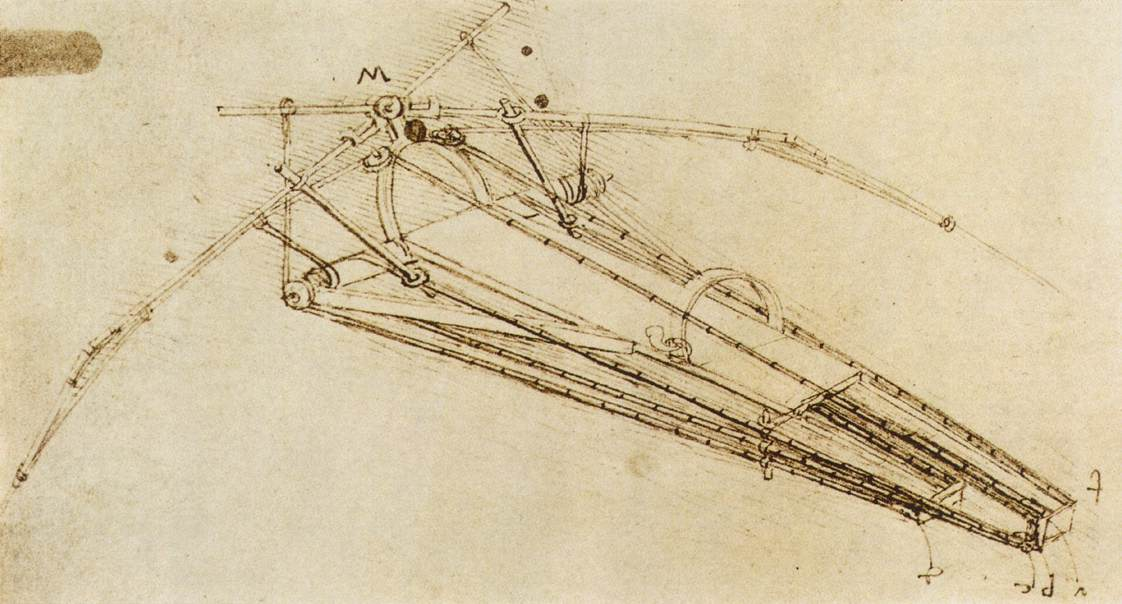
\includegraphics[height=50mm]{fig5/historical-davinci.jpg} \\
	\scriptsize Leonardo da Vinci and Flight \\
	\tiny (National Air and Space Museum, Smithsonian)
\end{center}
\vfill
\end{frame}


\begin{frame}
\frametitle{Historische Visualisierung}

\vfill
\begin{center}
	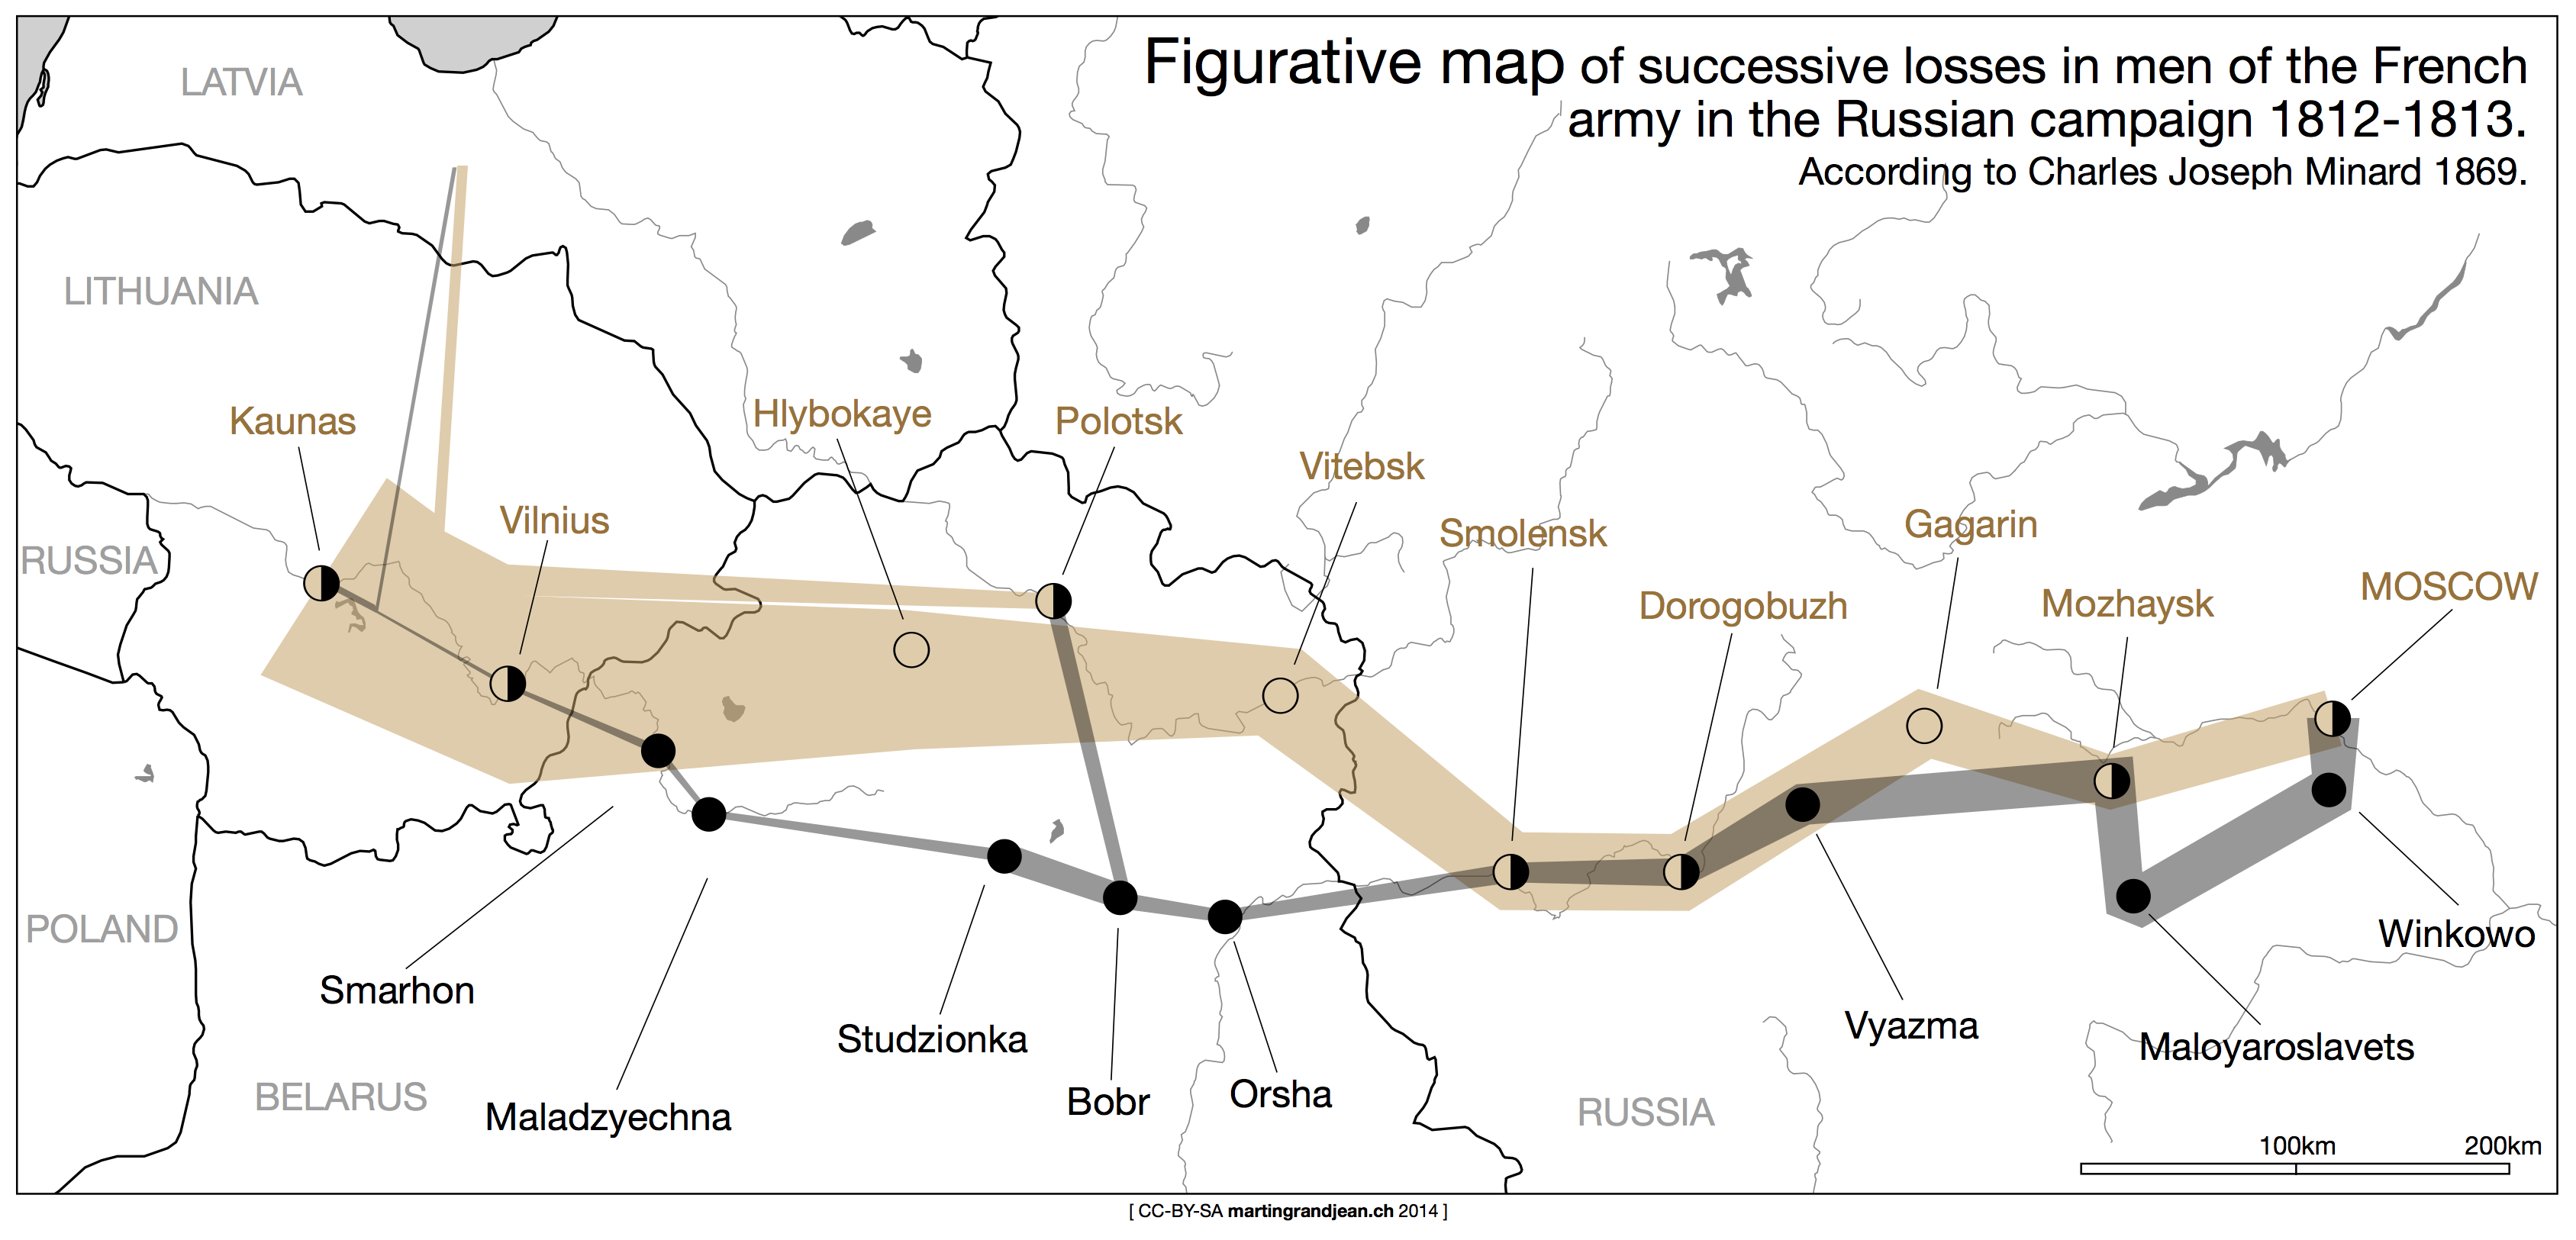
\includegraphics[height=50mm]{fig5/historical-napoleon.png}
\end{center}
\vfill
\end{frame}


\begin{frame}
\frametitle{Historische Visualisierung}

\vfill
\begin{center}
	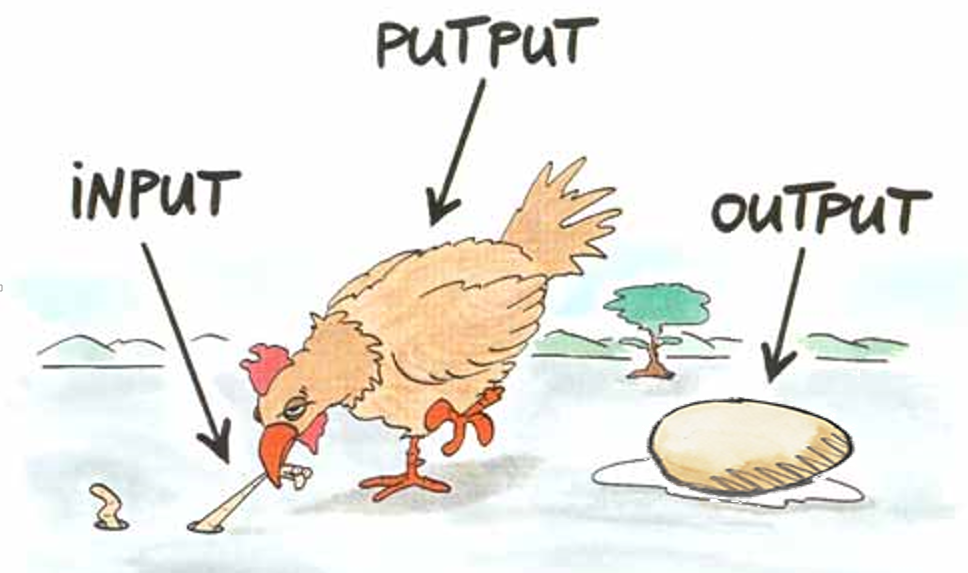
\includegraphics[height=50mm]{fig5/historical-putput.png} \\
	\scriptsize Output-Orientierung in den Bildungswissenschaften
\end{center}
\vfill
\end{frame}


\begin{frame}
\frametitle{Historische Visualisierung}

\vfill
\begin{center}
	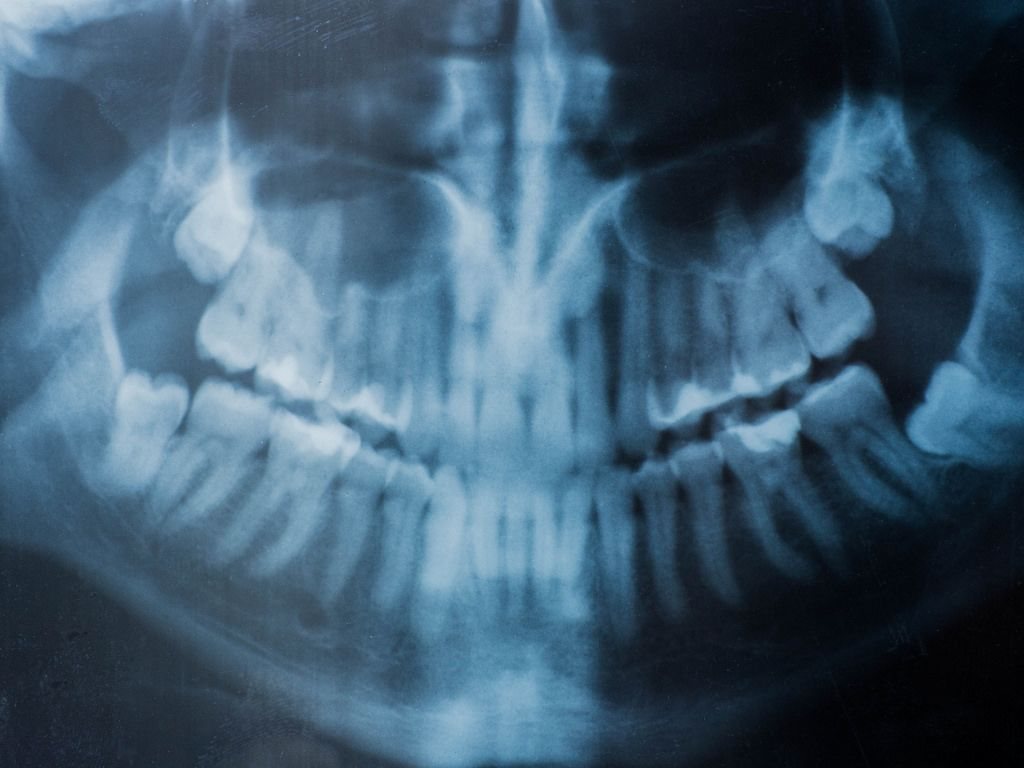
\includegraphics[height=50mm]{fig5/historical-roentgen.jpg} \\
	\scriptsize Röntgenbild eines menschlichen Kiefers mit Zähnen \\
	\tiny (Marco Verch, Creative Commons 2.0)
\end{center}
\vfill
\end{frame}


\begin{frame}
\frametitle{Historische Visualisierung}

\vfill
\begin{center}
	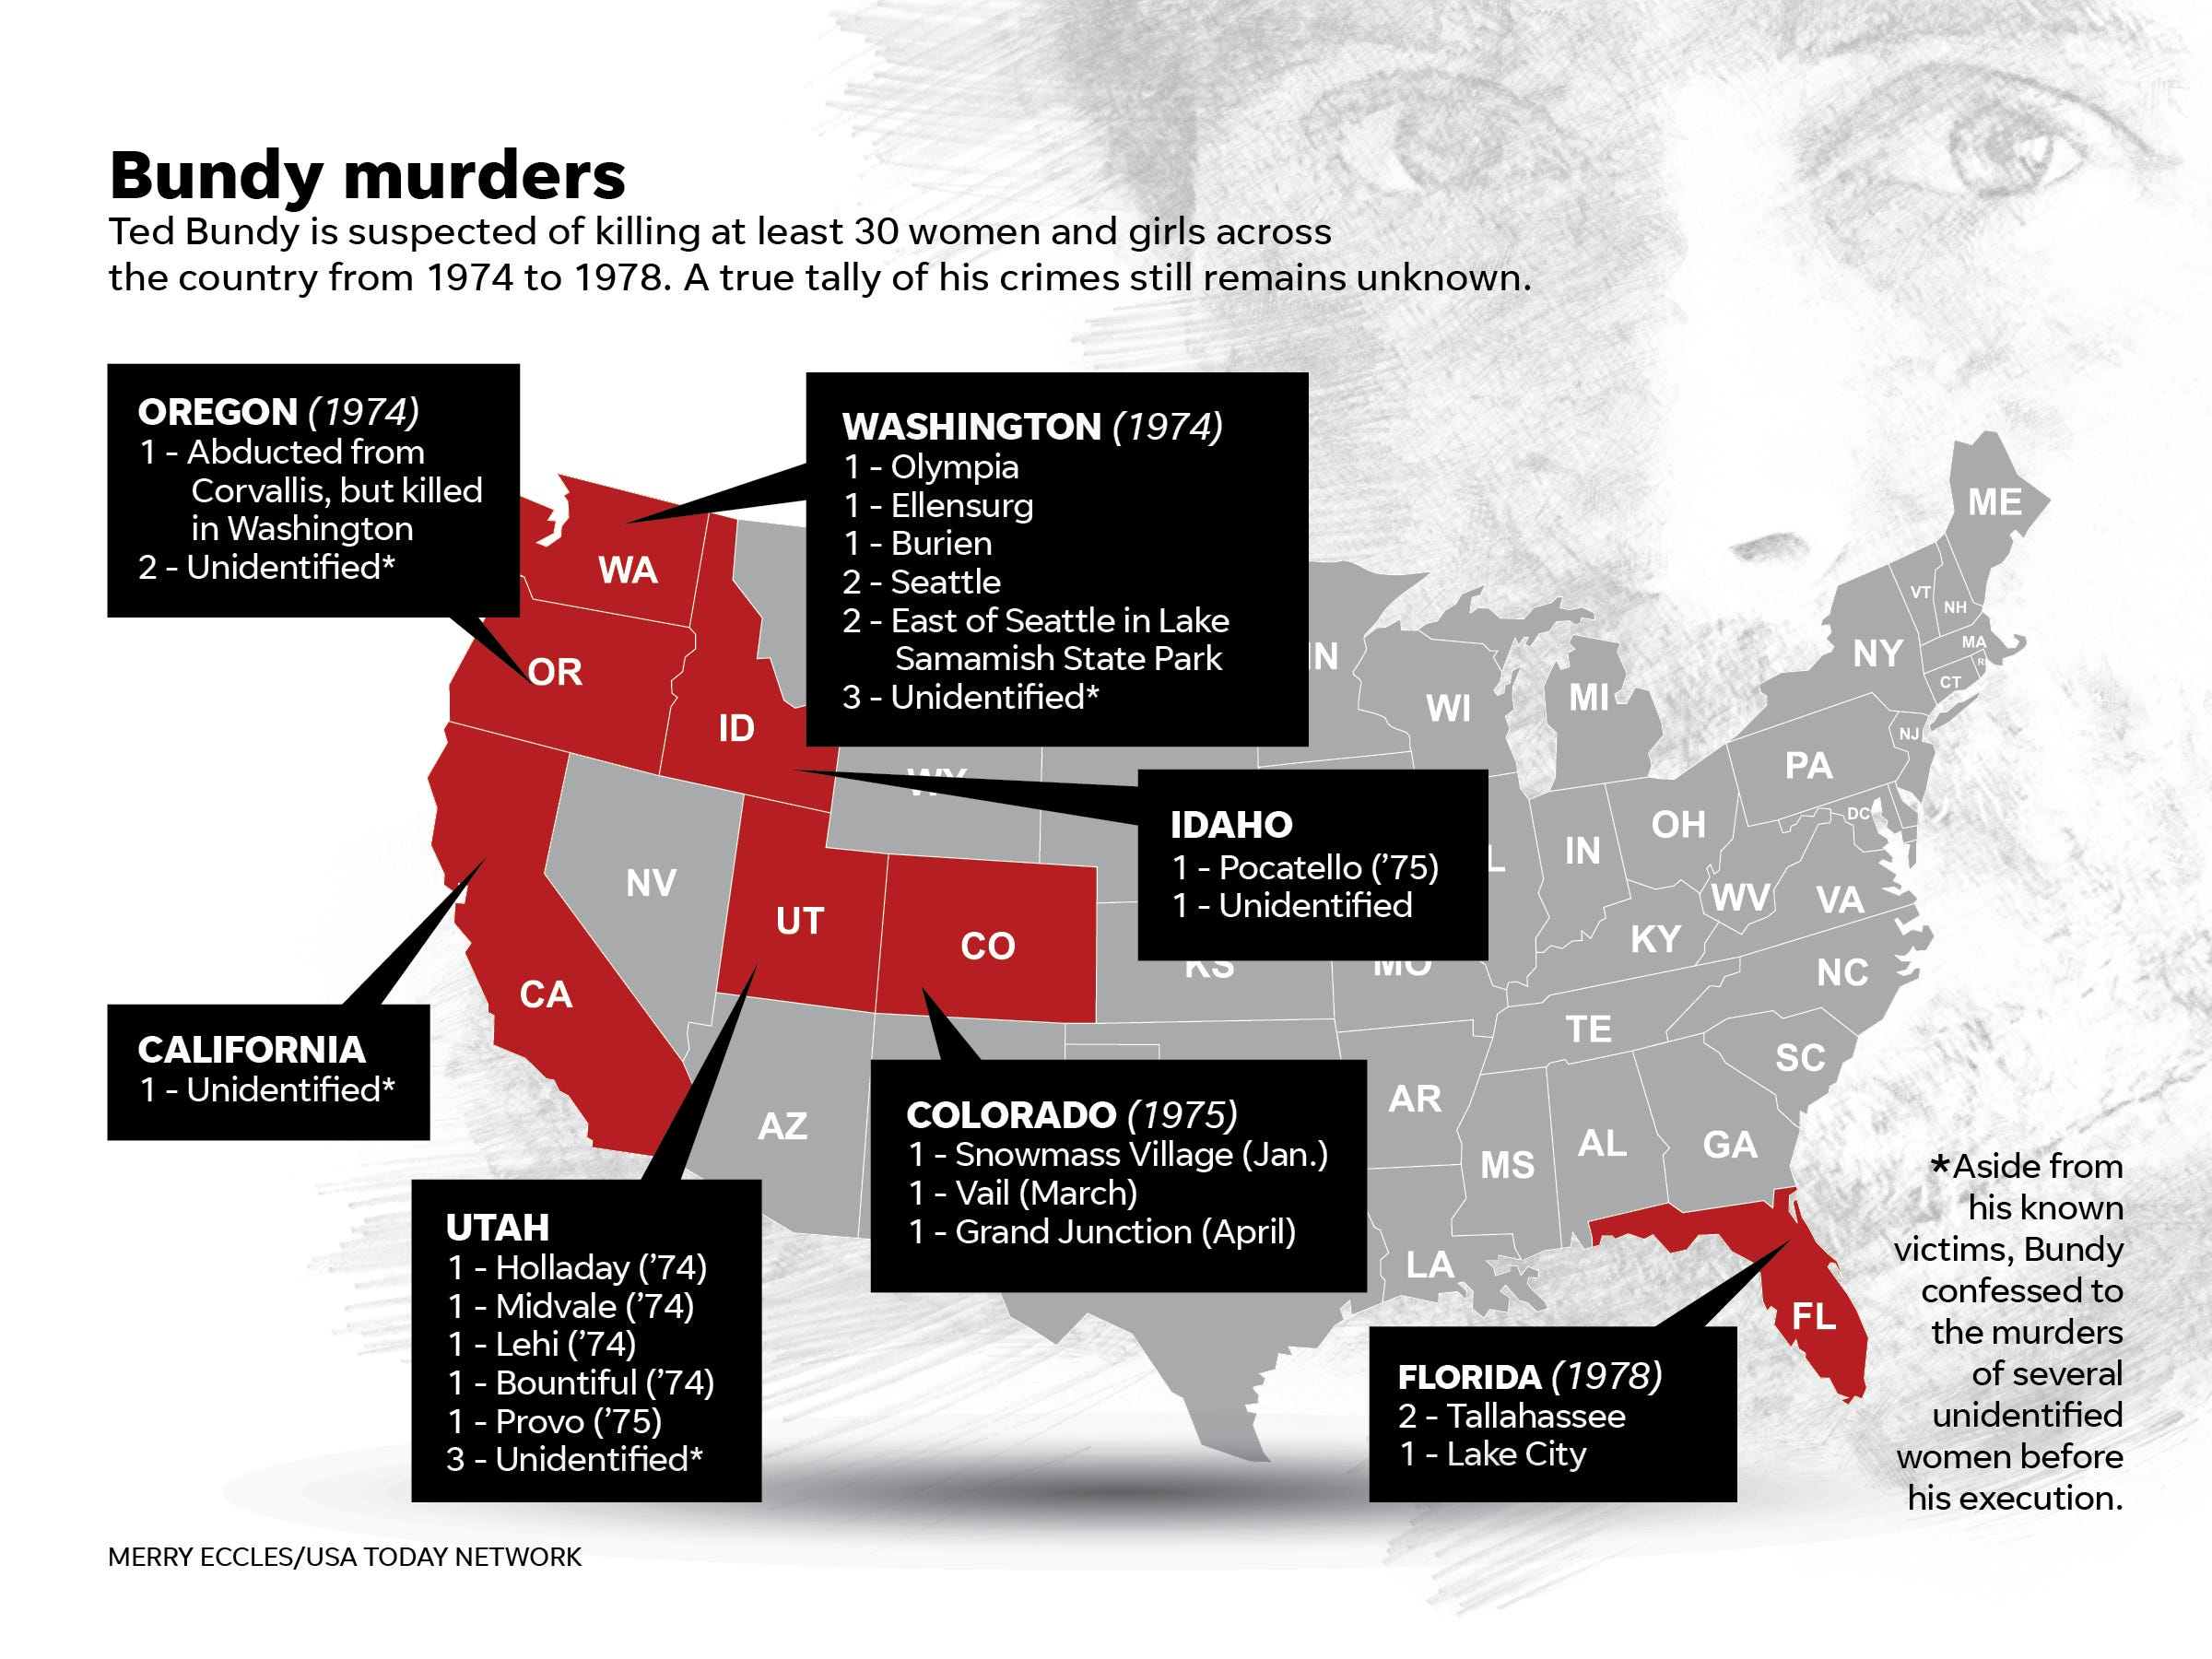
\includegraphics[height=70mm]{fig5/historical-tedbundy.jpg}
\end{center}
\vfill
\end{frame}


\begin{frame}
\frametitle{Historische Visualisierung}

\vfill
\begin{center}
	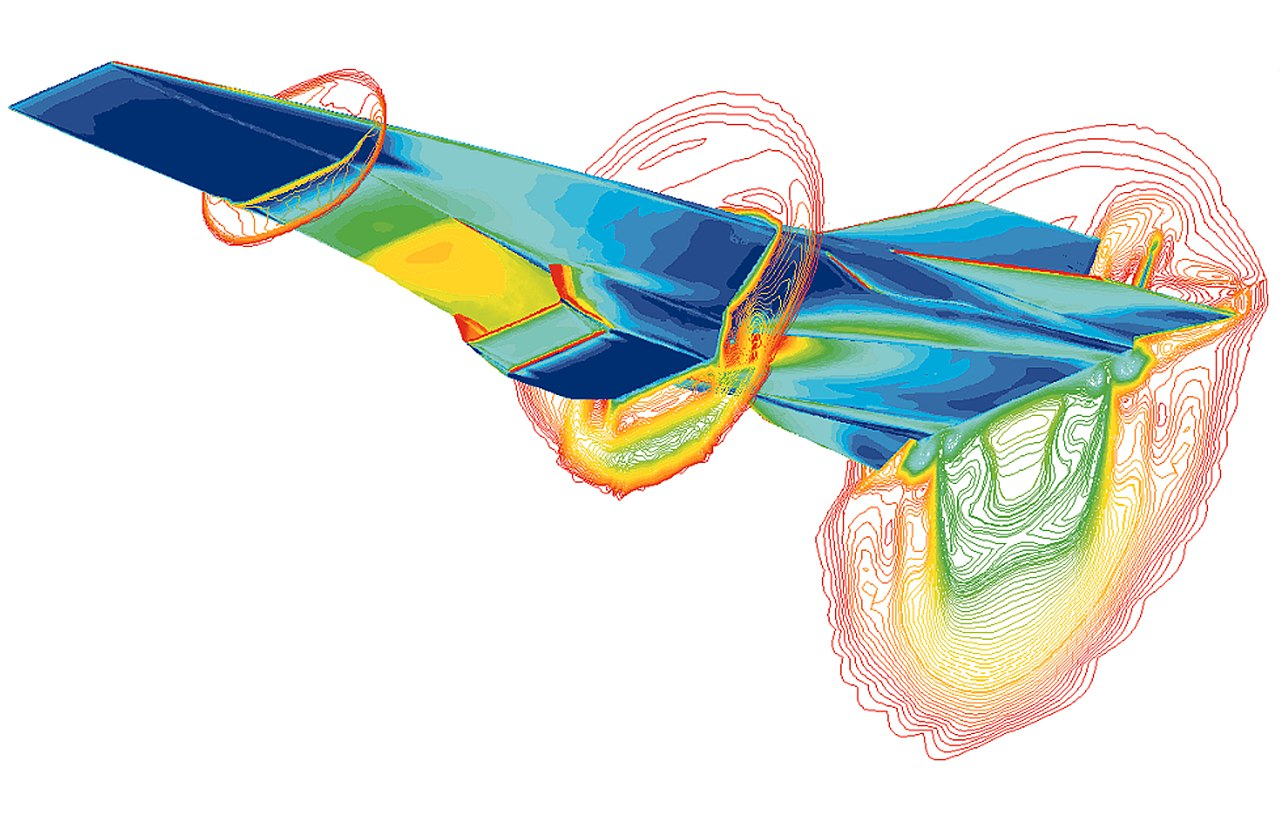
\includegraphics[height=50mm]{fig5/historical-nasa.jpg} \\
	\scriptsize Visualisierung einer CFD-Simulation der Boeing X-43 bei Mach 7 \\
	\tiny (NASA, gemeinfrei)
\end{center}
\vfill
\end{frame}


%\begin{frame}
%\frametitle{Datenvisualisierung in der Data Science}
%
%\begin{itemize}
%	\item von \sout{abstrakten Konstrukten} Zahlen zu Bildern
%\end{itemize}
%\end{frame}


\begin{frame}[fragile]
\frametitle{Aus der Data Science: Trend}

\begin{minted}[fontsize=\scriptsize]{python}
m = df.groupby('release_year').size()
m.idxmax(), m.loc[m.idxmax()]
# (2021, 125)

nbins = int(df['release_year'].max() - df['release_year'].min() + 1)
px.histogram(df, x='release_year', nbins=nbins)
\end{minted}

\begin{center}
	\vspace{-\baselineskip}
	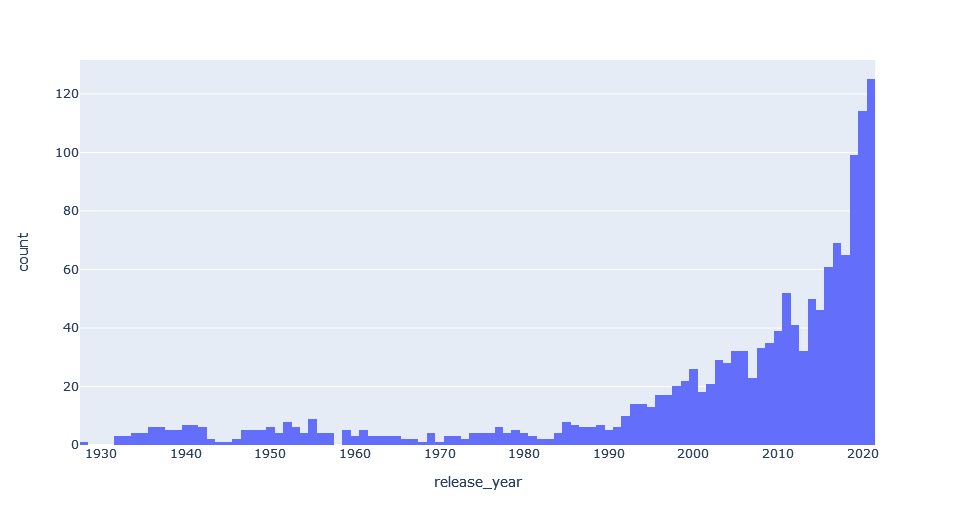
\includegraphics[height=0.5\textheight]{fig5/histogram1.png}
\end{center}
\end{frame}


\begin{frame}[fragile]
\frametitle{Aus der Data Science: Ausreißer}

\begin{minted}[fontsize=\scriptsize]{python}
m = df.groupby('date_added').size()
m.idxmax(), m.loc[m.idxmax()]
# (Timestamp('2019-11-12 00:00:00'), 722)

px.histogram(df, x='date_added')
\end{minted}

\begin{center}
	\vspace{-\baselineskip}
	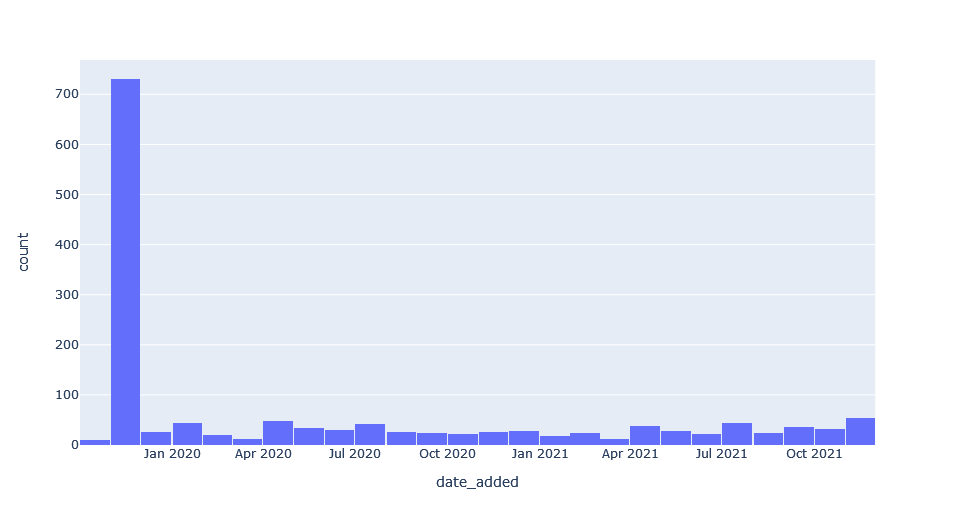
\includegraphics[height=0.5\textheight]{fig5/histogram2.png}
\end{center}
\end{frame}


\begin{frame}
\frametitle{Aus der Data Science: Cluster}

\vfill

\begin{minipage}{0.35\textwidth}
	\begin{center}
		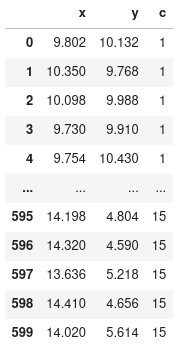
\includegraphics[height=50mm]{fig5/clustering-table.png}
	\end{center}
\end{minipage}%
\begin{minipage}{0.65\textwidth}
	\begin{center}
		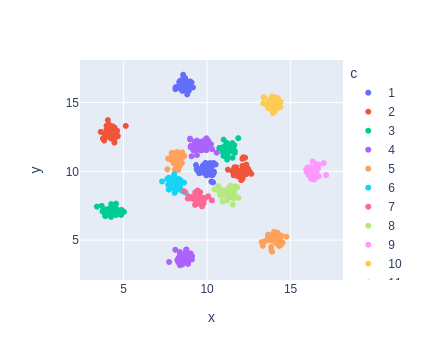
\includegraphics[height=50mm, clip, trim=5mm 6mm 0mm 14mm]{fig5/clustering-plot.png}
	\end{center}
\end{minipage}

\vfill
\end{frame}


\begin{frame}
\frametitle{Aus der Data Science: Graph}

\vfill
\begin{center}
	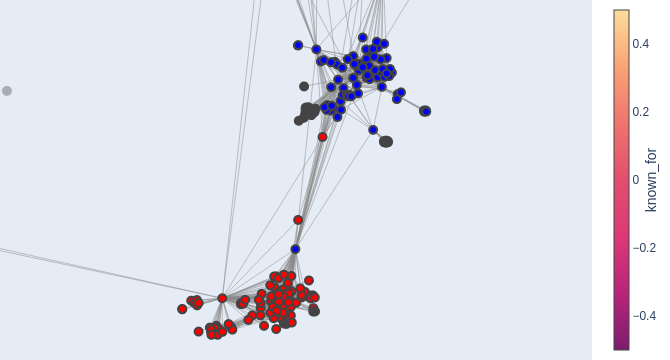
\includegraphics[height=50mm]{fig5/graph.png}
\end{center}
\vfill
\end{frame}



%%%%%%%%%%%%%%%%%%%%%%%%%%%%%%%%%%%%%%%%%%%%%%%%%%%%%%%%%%%%%%%%%%%%%%%%%%%%%%%%
% Prinzipien der Visualisierung                                                %
%%%%%%%%%%%%%%%%%%%%%%%%%%%%%%%%%%%%%%%%%%%%%%%%%%%%%%%%%%%%%%%%%%%%%%%%%%%%%%%%
\section{Prinzipien der Visualisierung}


\begin{frame}
\frametitle{Prinzipien der Visualisierung}

\begin{itemize}
	\item Mayer, R. E. (2001): Multimedia Learning. Cambridge: University Press.
	\item eigentlich \textit{Prinzipien des multimedialen \hl{Lernens}}
	\item wichtige Tipps zur Gestaltung und Präsentation von Darstellungen
\end{itemize}
\end{frame}


\begin{frame}
\frametitle{1. Multimediaprinzip}

\begin{itemize}
	\item Kombination von Text / Erklärung und Grafik
	\item Grafiken zeigen Beziehungen zwischen Informationen
\end{itemize}
\end{frame}


\begin{frame}
\frametitle{2. Kontiguitätsprinzip}

\begin{itemize}
	\item zeitgleiche Darstellung von Wort und Bild
	\item räumlich zusammenhängend
	\item Sprünge (insbesondere über Seitenumbrüche hinweg) und Scrollen \textbf{vermeiden}
\end{itemize}
\end{frame}


\begin{frame}
\frametitle{3. Kohärenzprinzip}

\begin{itemize}
	\item \textit{Weniger ist mehr!}
	\item Überfrachtung wirkt kontraproduktiv
	\item irrelevante Inhalte entfernen oder verlagern
\end{itemize}
\end{frame}


\begin{frame}
\frametitle{4. Modalitätsprinzip}

\begin{itemize}
	\item gesprochener Text zur Erläuterung besser als geschriebener
	\item insbesondere bei bewegten Bildern
	% \item Gestaltung der Ergebnispräsentation
\end{itemize}
\end{frame}


\begin{frame}
\frametitle{5. Redundanzprinzip}

\begin{itemize}
	\item gleiche Information als Bild, Ton und Text vermeiden
	\item Informationen sollen einander ergänzen, nicht ersetzen
	\item Stärken der einzelnen Darstellungsformen beachten
\end{itemize}

\vspace{1cm}

\begin{itemize}
	\item {\color{gray} Schreiben Sie nicht alles auf Ihre Folien, was Sie sowieso sagen werden.}
	\item {\color{lightgray} \dots{} außer es ist ein Handout und dient Ihren Zuhörern bei der Prüfungsvorbereitung!}
\end{itemize}
\end{frame}


\begin{frame}
\frametitle{6. Personalisierungsprinzip}

\begin{itemize}
	\item Ausrichtung auf Adressaten
	\begin{itemize}
		\item Vorwissen
		\item Empfangsweg (digital, gedruckt, präsentiert, \dots)
		\item institutionelle Rahmenbedingungen
		\item \dots
	\end{itemize}
	\item \textit{Abholen} des Lernenden / Zuhörers / etc.
	\item Erhaltung der Motivation
\end{itemize}
\end{frame}



%%%%%%%%%%%%%%%%%%%%%%%%%%%%%%%%%%%%%%%%%%%%%%%%%%%%%%%%%%%%%%%%%%%%%%%%%%%%%%%%
% Visualisierung mit Python                                                    %
%%%%%%%%%%%%%%%%%%%%%%%%%%%%%%%%%%%%%%%%%%%%%%%%%%%%%%%%%%%%%%%%%%%%%%%%%%%%%%%%
\section{Visualisierung mit Python}


\begin{frame}[fragile]
\frametitle{Python-Bibliotheken zur Visualisierung}

\begin{itemize}
	\item Matplotlib - Visualization with Python
	\item seaborn: statistical data visualization
	\item \hl{Plotly.py} - Plotly Python Graphing Library
\end{itemize}

\begin{minted}{python}
import plotly.express as px

px.bar(df, x='attr_x', y='attr_y',
       title='Produktionen pro Jahr',
       labels={'attr_x': 'X Werte', 'attr_y': 'Y Werte'})
\end{minted}
\end{frame}


\begin{frame}
\frametitle{Histogramme}

\begin{itemize}
	\item eine Art Säulendiagramm
	\item relative und absolute Häufigkeiten
	\item Klasseneinteilung in sog. \alert{Bins} (Behälter)
\end{itemize}
\end{frame}


\begin{frame}[fragile]
\frametitle{Histogramme}

\begin{minted}{python}
import plotly.express as px
px.histogram(df, x='release_year', nbins=nbins)
\end{minted}

\begin{minipage}{0.5\textwidth}%
\begin{center}%
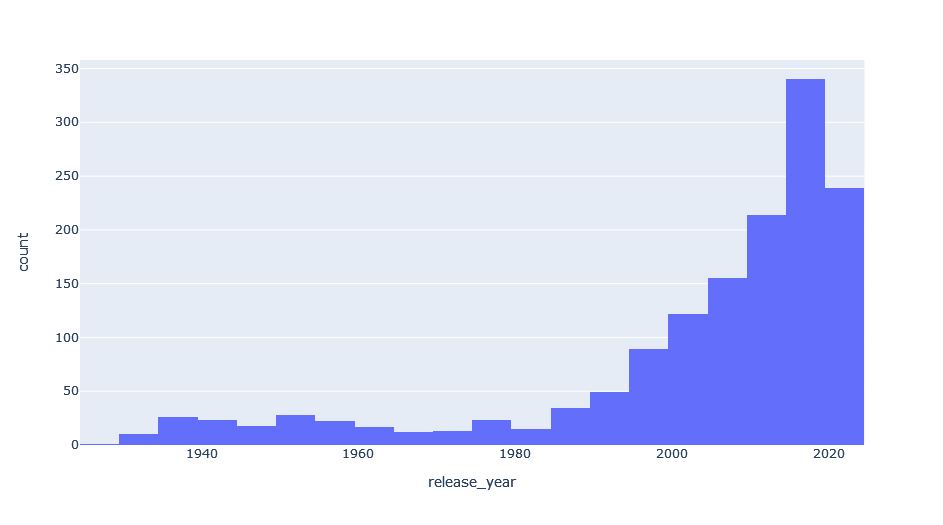
\includegraphics[width=\linewidth]{fig5/histogram3.png}%
\end{center}%
\end{minipage}%
\begin{minipage}{0.5\textwidth}%
\begin{center}%
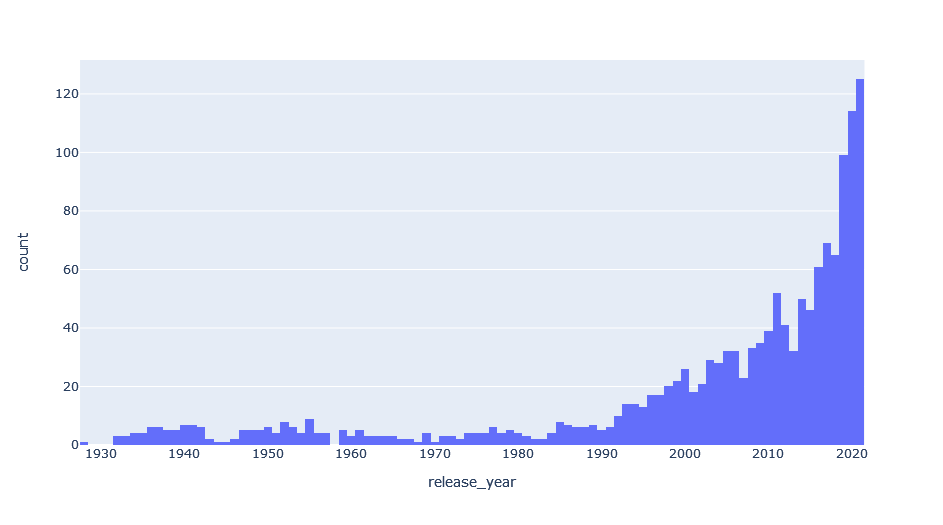
\includegraphics[width=\linewidth]{fig5/histogram4.png}%
\end{center}%
\end{minipage}%
\end{frame}


\begin{frame}
\frametitle{Liniendiagramme}

\begin{itemize}
\item Menge von Punkten durch Linie verbunden
\item suggeriert Kontinuität (stetige Funktionen bevorzugt!)
\end{itemize}
\end{frame}


\begin{frame}[fragile]
\frametitle{Liniendiagramme}

\begin{minted}{python}
import plotly.express as px
px.line(df, x='year', y='total_assets')
\end{minted}

\vspace{-\baselineskip}

\begin{center}
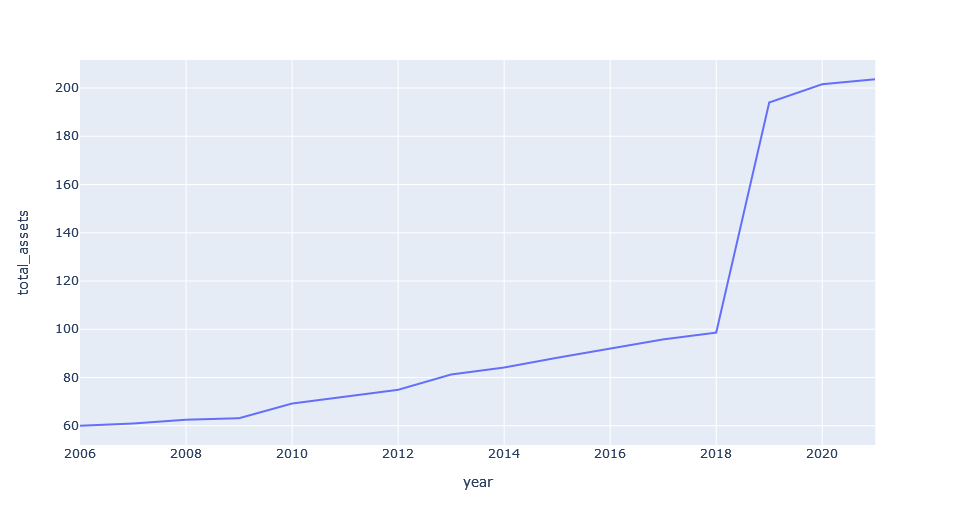
\includegraphics[width=0.85\linewidth]{fig5/line1.png}
\end{center}
\end{frame}


\begin{frame}
\frametitle{Balken- und Säulendiagramme}

\begin{itemize}
\item \textit{vergleichende} Diagramme
\item Höhe der Balken proportional zur Ausprägung des Merkmals
\item in seltenen Fällen auch die Fläche
\end{itemize}
\end{frame}


\begin{frame}[fragile]
\frametitle{Balken- und Säulendiagramme}

\begin{minted}{python}
import plotly.express as px
px.bar(df, x='country', y='movies')
\end{minted}

\vspace{-\baselineskip}

\begin{center}
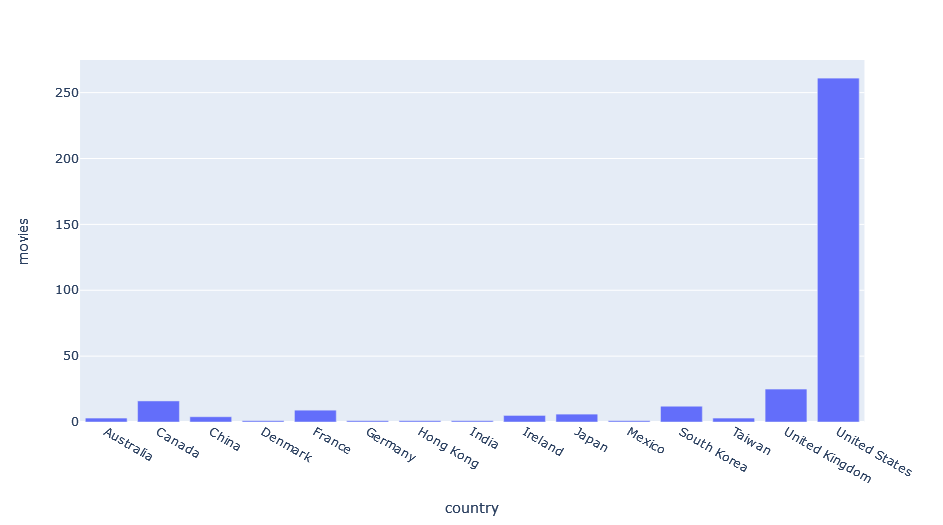
\includegraphics[width=0.85\linewidth]{fig5/bar1.png}
\end{center}
\end{frame}


\begin{frame}[fragile]
\frametitle{Balken- und Säulendiagramme}

\begin{minted}{python}
import plotly.express as px
px.bar(df, x='country', y='movies', orientation='h')
\end{minted}

\vspace{-\baselineskip}

\begin{center}
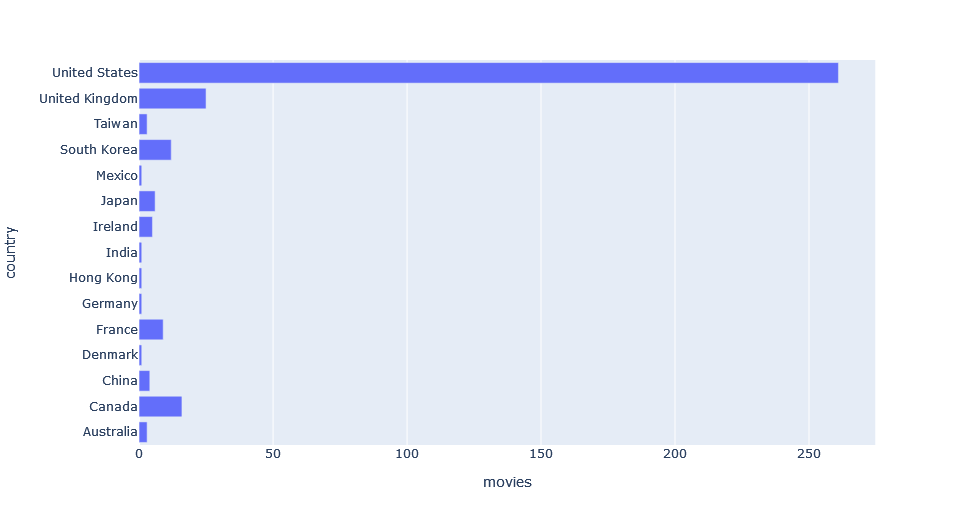
\includegraphics[width=0.85\linewidth]{fig5/bar2.png}
\end{center}
\end{frame}


\begin{frame}[fragile]
\frametitle{Balken- und Säulendiagramme}

\begin{minted}{python}
import plotly.express as px
px.bar(df, x='country', y=['movies', 'tvshows'], log_y=True,
       barmode=...)
\end{minted}

\begin{minipage}{0.5\textwidth}%
\begin{center}%
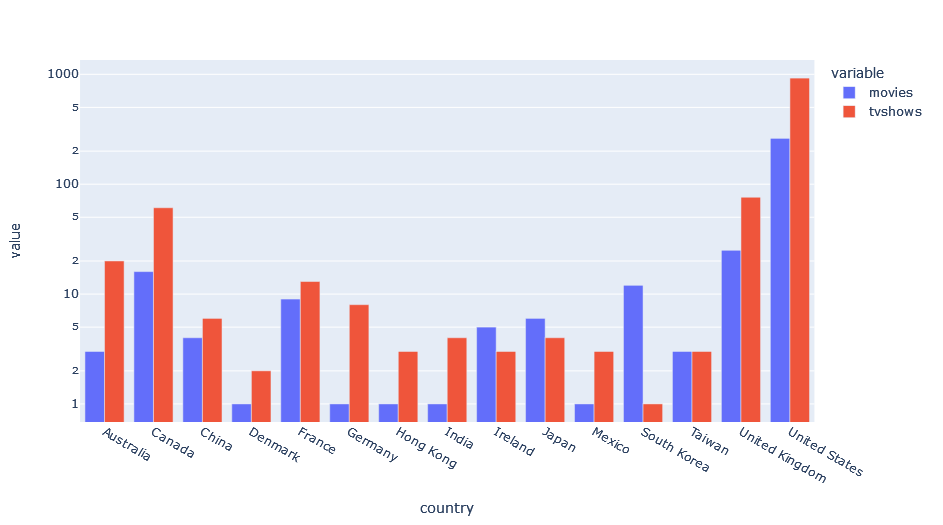
\includegraphics[width=\linewidth]{fig5/bar3.png}%
\end{center}%
\end{minipage}%
\begin{minipage}{0.5\textwidth}%
\begin{center}%
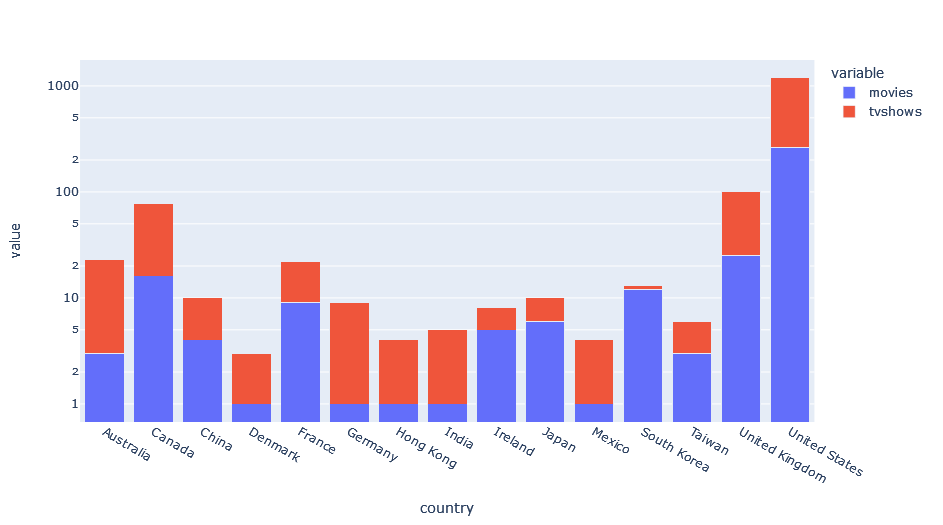
\includegraphics[width=\linewidth]{fig5/bar4.png}%
\end{center}%
\end{minipage}%

\begin{minipage}{0.5\textwidth}%
\begin{center}%
\scriptsize \textit{group}
\end{center}%
\end{minipage}%
\begin{minipage}{0.5\textwidth}%
\begin{center}%
\scriptsize \textit{stack}
\end{center}%
\end{minipage}%
\end{frame}


\begin{frame}[fragile]
\frametitle{Balken- und Säulendiagramme}

\begin{minted}{python}
import plotly.express as px
px.bar(df, x='release_year', y='duration', error_y='sem')
\end{minted}

\vspace{-\baselineskip}

\begin{center}
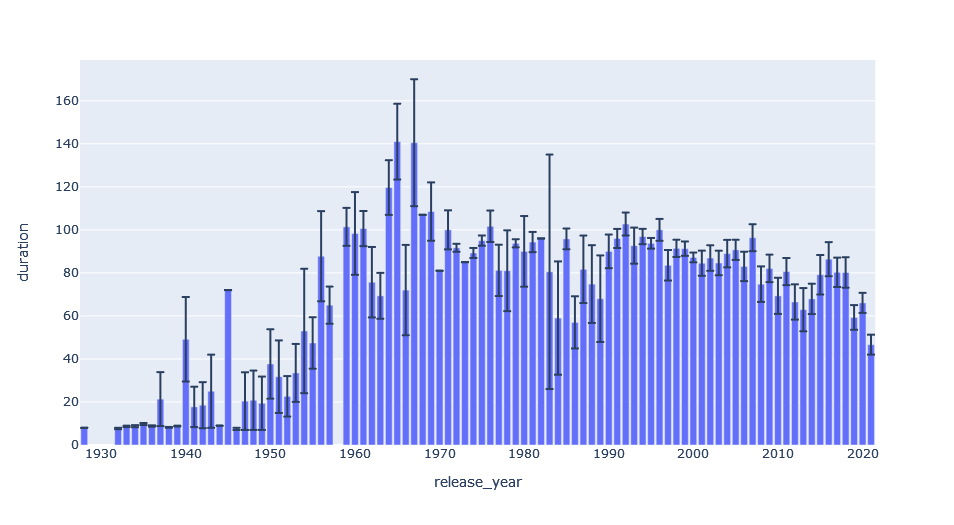
\includegraphics[width=0.85\linewidth]{fig5/bar5.png}
\end{center}
\end{frame}


\begin{frame}
\frametitle{Kreisdiagramme}

\begin{itemize}
\item Darstellung relativer Anteile
\item dreidimensional als Kuchen- oder Tortendiagramm
\end{itemize}

\begin{center}
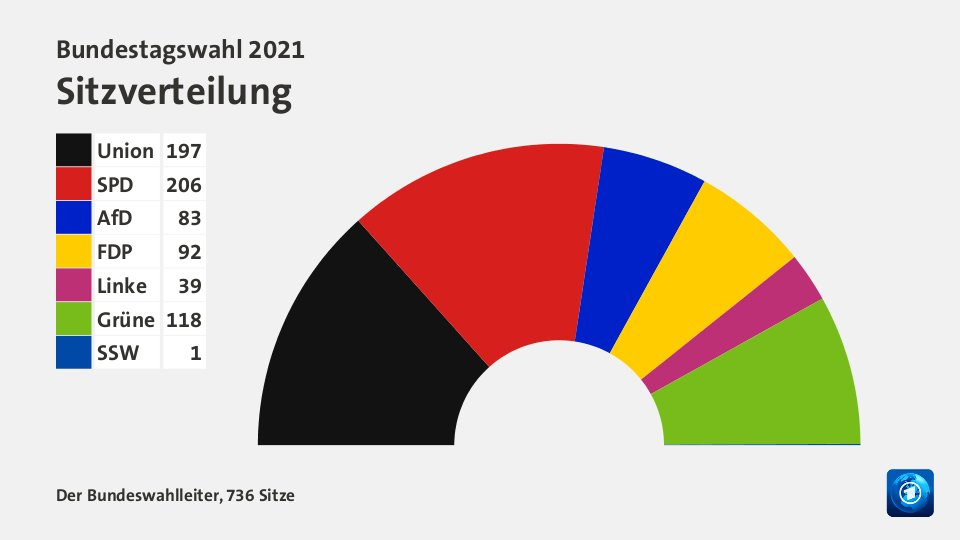
\includegraphics[width=0.85\linewidth]{fig5/pie1.jpg}
\end{center}
\end{frame}


\begin{frame}[fragile]
\frametitle{Kreisdiagramme}

\begin{minted}{python}
import plotly.express as px
px.pie(df, values='count', names='name')
\end{minted}

\vspace{-\baselineskip}

\begin{center}
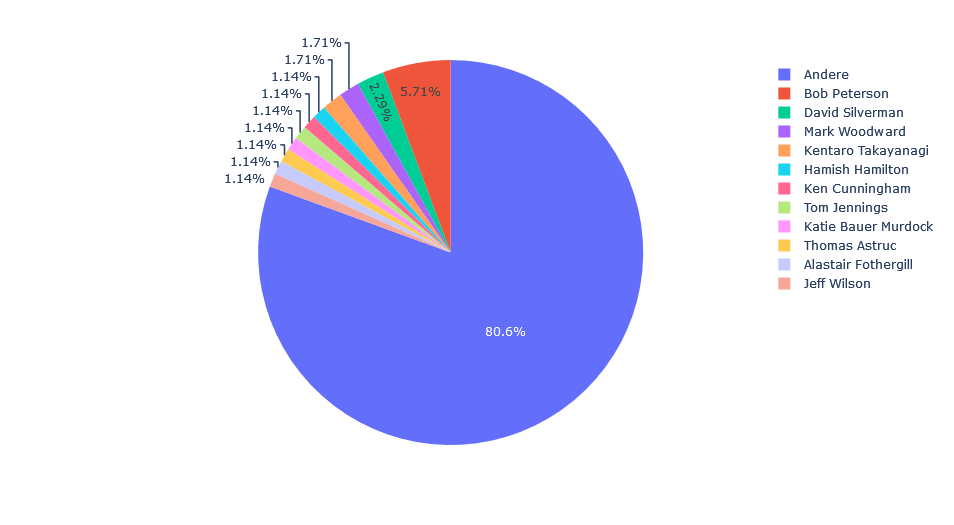
\includegraphics[width=0.85\linewidth]{fig5/pie2.png}
\end{center}
\end{frame}


\begin{frame}[fragile]
\frametitle{Kreisdiagramme}

\begin{minted}{python}
import plotly.express as px
px.pie(df, values='count', names='name',
       hole=0.5)
\end{minted}

\vspace{-\baselineskip}

\begin{center}
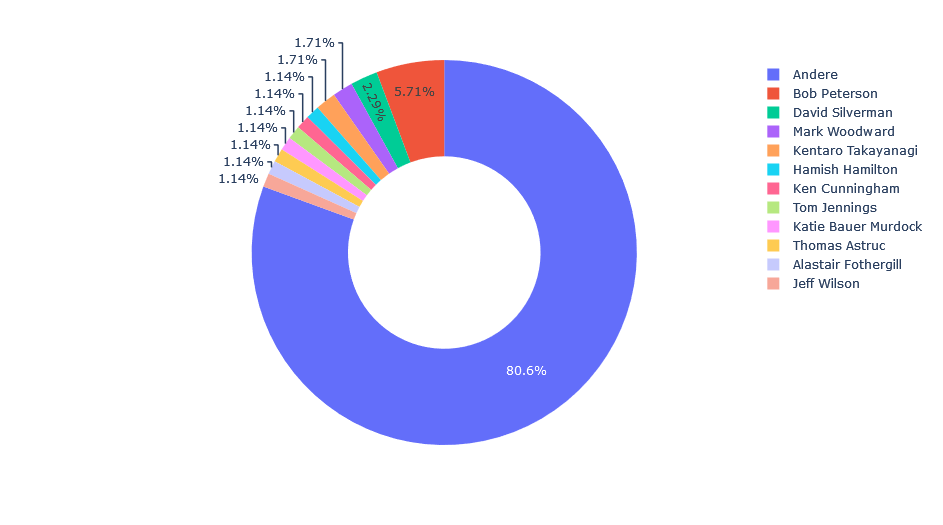
\includegraphics[width=0.85\linewidth]{fig5/pie3.png}
\end{center}
\end{frame}


\begin{frame}[fragile]
\frametitle{Kreisdiagramme}

\begin{minted}{python}
import plotly.express as px
fig = px.pie(df, names='type', values='count')
fig.update_traces(pull=[0.25, 0, 0])
\end{minted}

\vspace{-\baselineskip}

\begin{center}
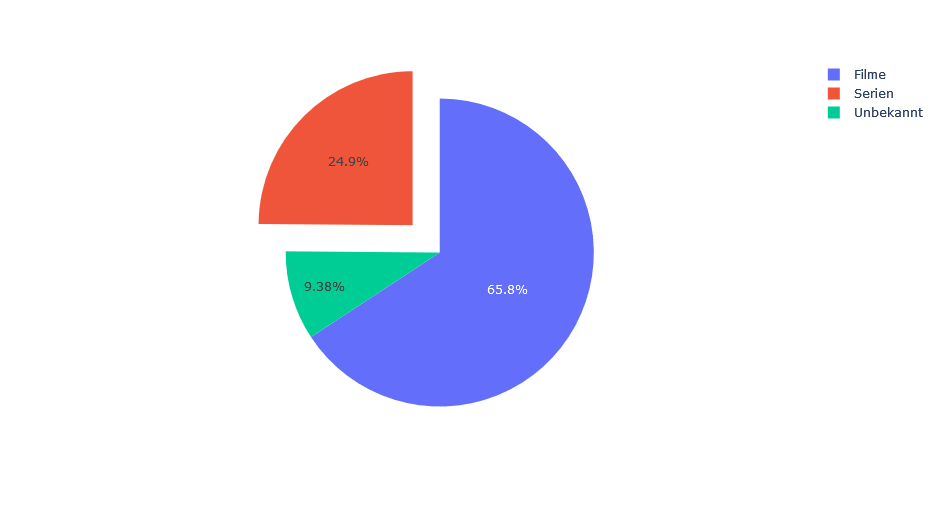
\includegraphics[width=0.80\linewidth]{fig5/pie4.png}
\end{center}
\end{frame}


\begin{frame}
\frametitle{Streudiagramme}

\begin{itemize}
	\item Punktwolke
	\item jedes Wertepaar einzeln
	\item Wiedererkennung statistischer Merkmale
\end{itemize}
\end{frame}


\begin{frame}[fragile]
\frametitle{Streudiagramme}

\begin{minted}{python}
import plotly.express as px
px.scatter(df, x='release_year', y='duration_in_minutes')
\end{minted}

\vspace{-\baselineskip}

\begin{center}
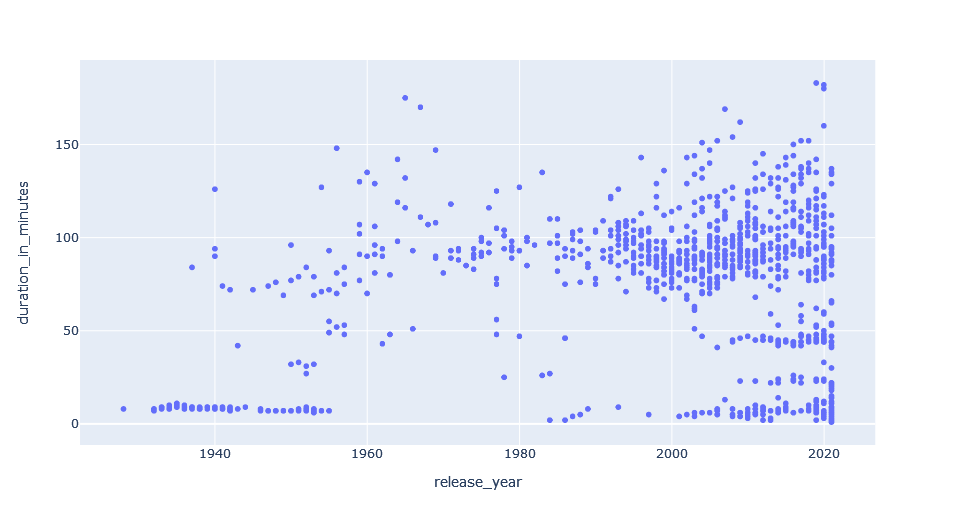
\includegraphics[width=0.80\linewidth]{fig5/scatter1.png}
\end{center}
\end{frame}


\begin{frame}[fragile]
\frametitle{Streudiagramme}

\begin{minted}{python}
import plotly.express as px
px.scatter(df, x='release_year', y='duration_in_minutes',
           size='cast_size')
\end{minted}

\vspace{-\baselineskip}

\begin{center}
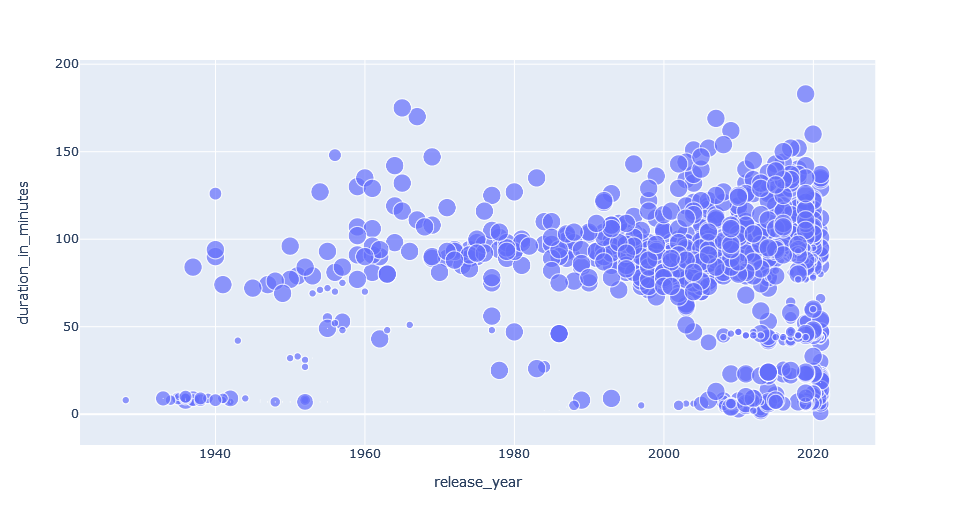
\includegraphics[width=0.80\linewidth]{fig5/scatter2.png}
\end{center}
\end{frame}


\begin{frame}[fragile]
\frametitle{Streudiagramme}

\begin{minted}{python}
import plotly.express as px
px.scatter(df, x='release_year', y='duration_in_minutes',
           color='cast_size')
\end{minted}

\vspace{-\baselineskip}

\begin{center}
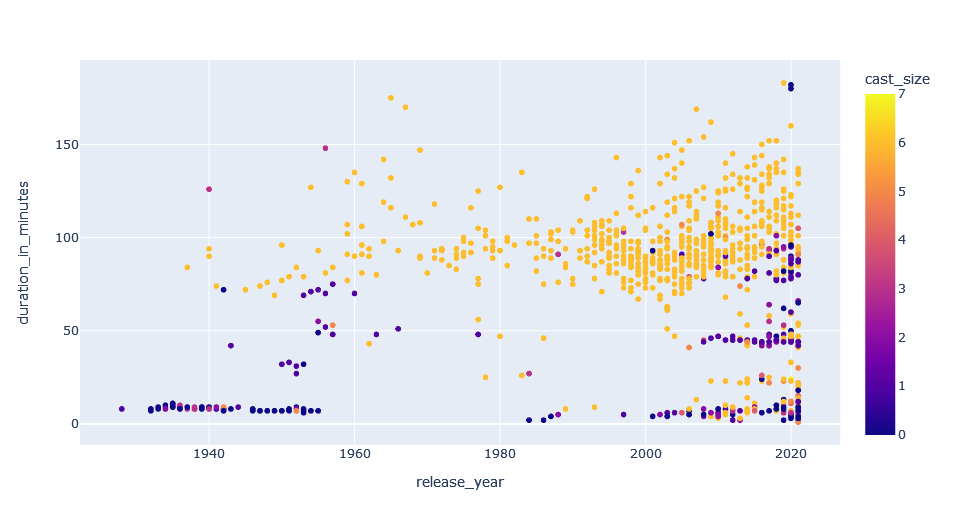
\includegraphics[width=0.80\linewidth]{fig5/scatter3.png}
\end{center}
\end{frame}


\begin{frame}[fragile]
\frametitle{Streudiagramme}

\begin{minted}{python}
import plotly.express as px
px.scatter(df, x='release_year', y='duration_in_minutes',
           symbol='director_size')
\end{minted}

\vspace{-\baselineskip}

\begin{center}
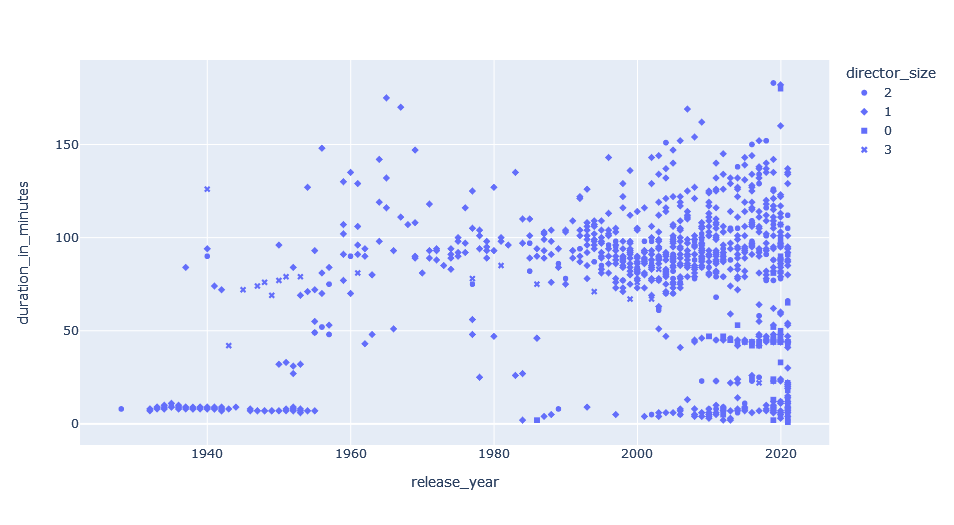
\includegraphics[width=0.80\linewidth]{fig5/scatter4.png}
\end{center}
\end{frame}


\begin{frame}
\frametitle{Streudiagramm-Matrix}

\begin{itemize}
	\item paarweise Streudiagramme
	\item Aufdecken statistischer Zusammenhänge
\end{itemize}
\end{frame}


\begin{frame}[fragile]
\frametitle{Streudiagramm-Matrix}

\begin{minted}{python}
import plotly.express as px
px.scatter_matrix(df[['date_added', 'release_year', 'rating', 'duration']])
\end{minted}

\vspace{-\baselineskip}

\begin{center}
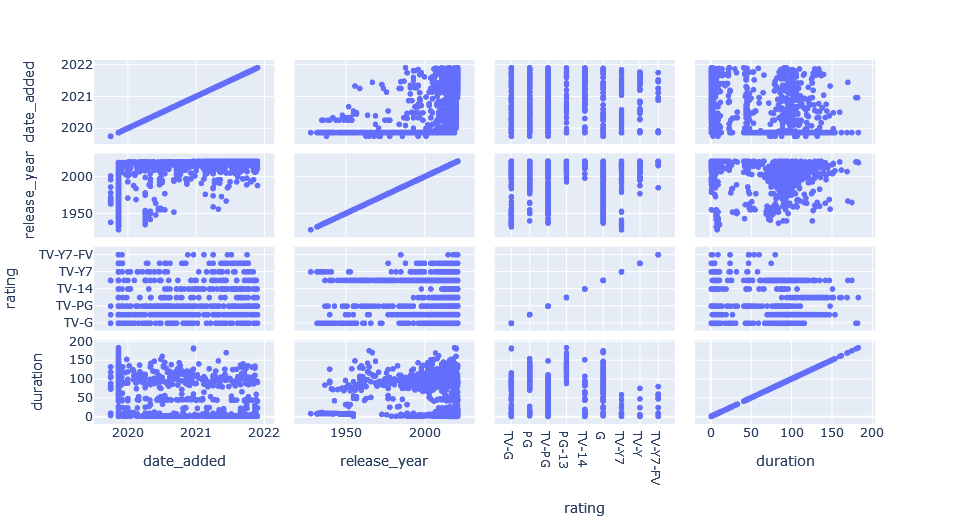
\includegraphics[width=0.80\linewidth]{fig5/matrix1.png}
\end{center}
\end{frame}


\begin{frame}
\frametitle{Streudiagramm-Matrix}

\begin{center}
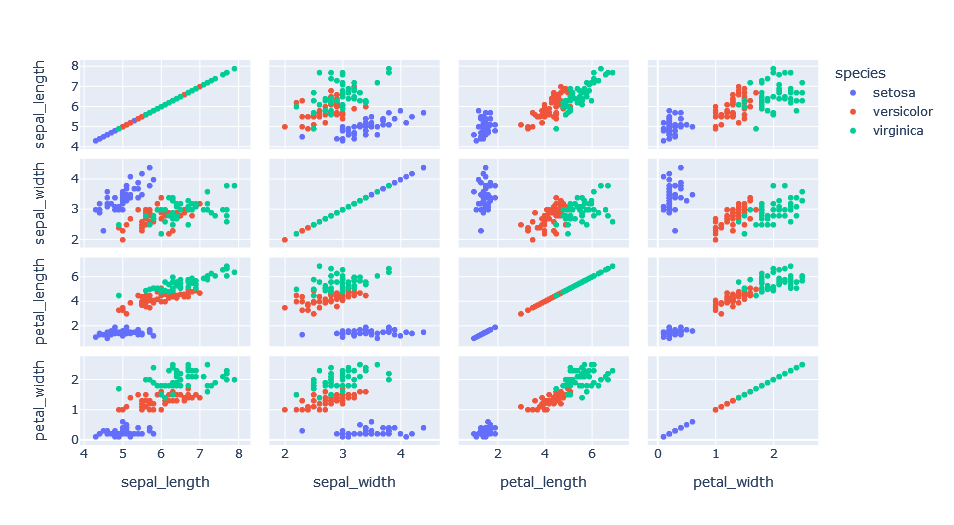
\includegraphics[width=\linewidth]{fig5/matrix2.png}
\end{center}
\end{frame}



%%%%%%%%%%%%%%%%%%%%%%%%%%%%%%%%%%%%%%%%%%%%%%%%%%%%%%%%%%%%%%%%%%%%%%%%%%%%%%%%
% Vertrauen Sie keiner Grafik                                                  %
%%%%%%%%%%%%%%%%%%%%%%%%%%%%%%%%%%%%%%%%%%%%%%%%%%%%%%%%%%%%%%%%%%%%%%%%%%%%%%%%
\section{Vertrauen Sie keiner Grafik}


%\begin{frame}
%\frametitle{Vertrauen Sie keiner Grafik}
%
%\dots{} deren Baseline Sie nicht selbst verschoben haben!
%\end{frame}


\begin{frame}
\frametitle{Verschieben der Baseline}

\vfill
\begin{center}
	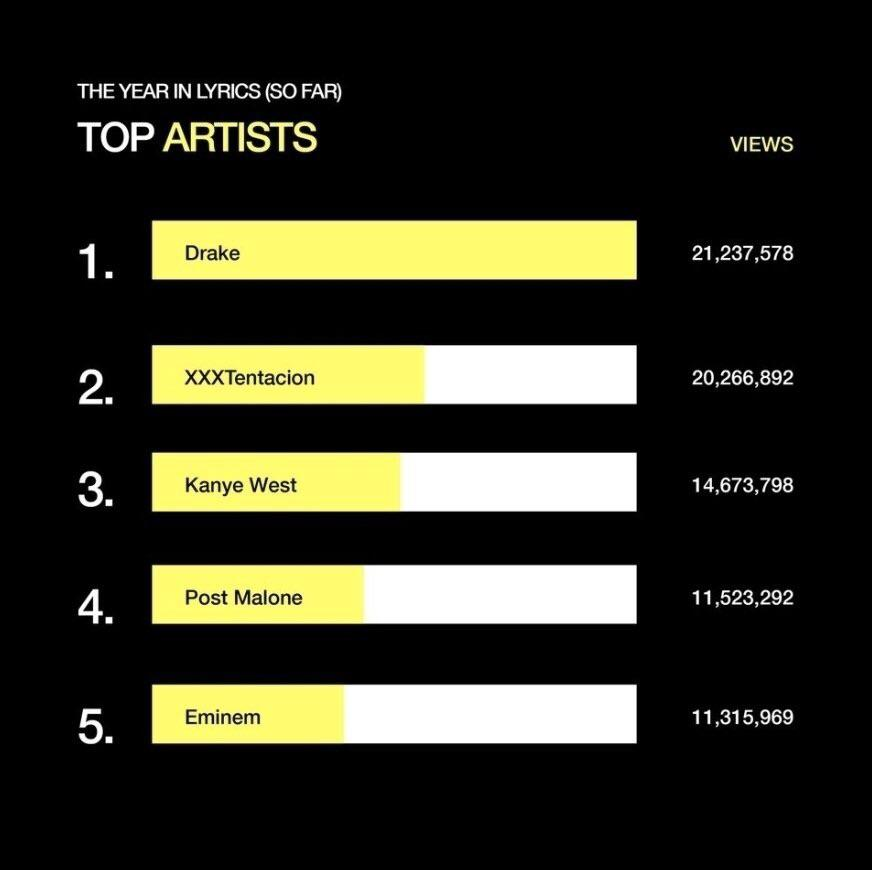
\includegraphics[height=60mm]{fig5/error-baseline1.jpg} \\
	\scriptsize \ehref{https://www.reddit.com/r/CrappyDesign/comments/8y0jxd}{reddit.com/r/CrappyDesign/comments/8y0jxd}
\end{center}
\vfill
\end{frame}


\begin{frame}
\frametitle{Verschieben der Baseline}

\vfill
\begin{center}
	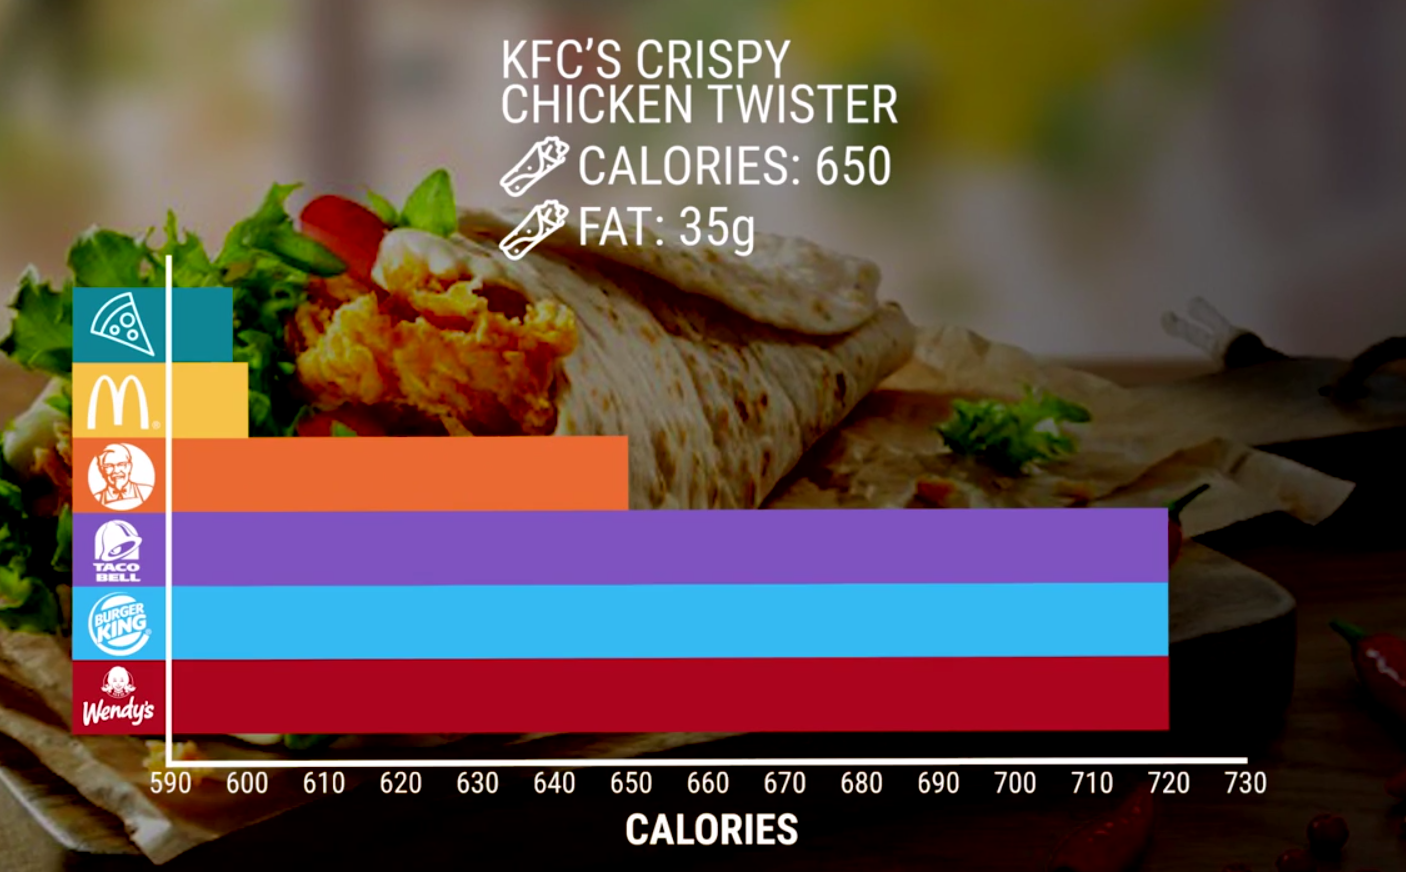
\includegraphics[height=60mm]{fig5/error-baseline2.png} \\
	\scriptsize \ehref{https://www.reddit.com/r/dataisugly/comments/6aaep3}{reddit.com/r/dataisugly/comments/6aaep3}
\end{center}
\vfill
\end{frame}


\begin{frame}
\frametitle{Verstoß gegen Konventionen}

\vfill
\begin{center}
	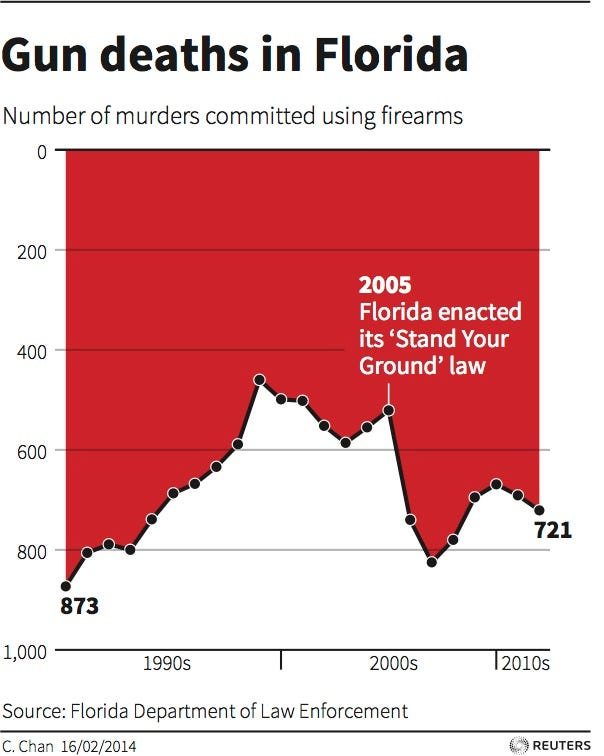
\includegraphics[height=60mm]{fig5/error-convention2.jpg} \\
	\scriptsize \ehref{https://www.businessinsider.com/gun-deaths-in-florida-increased-with-stand-your-ground-2014-2}{businessinsider.com}
\end{center}
\vfill
\end{frame}


\begin{frame}
\frametitle{Faxen mit Achsen}

\vfill
\begin{center}
	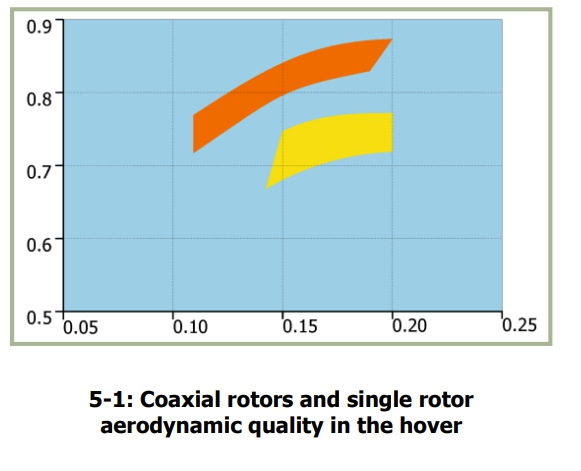
\includegraphics[height=60mm]{fig5/error-axis2.jpg} \\
	\scriptsize \ehref{https://www.reddit.com/r/dataisugly/comments/13jzvs9}{reddit.com/r/dataisugly/comments/13jzvs9}
\end{center}
\vfill
\end{frame}


\begin{frame}
\frametitle{Faxen mit Achsen}

\vfill
\begin{center}
	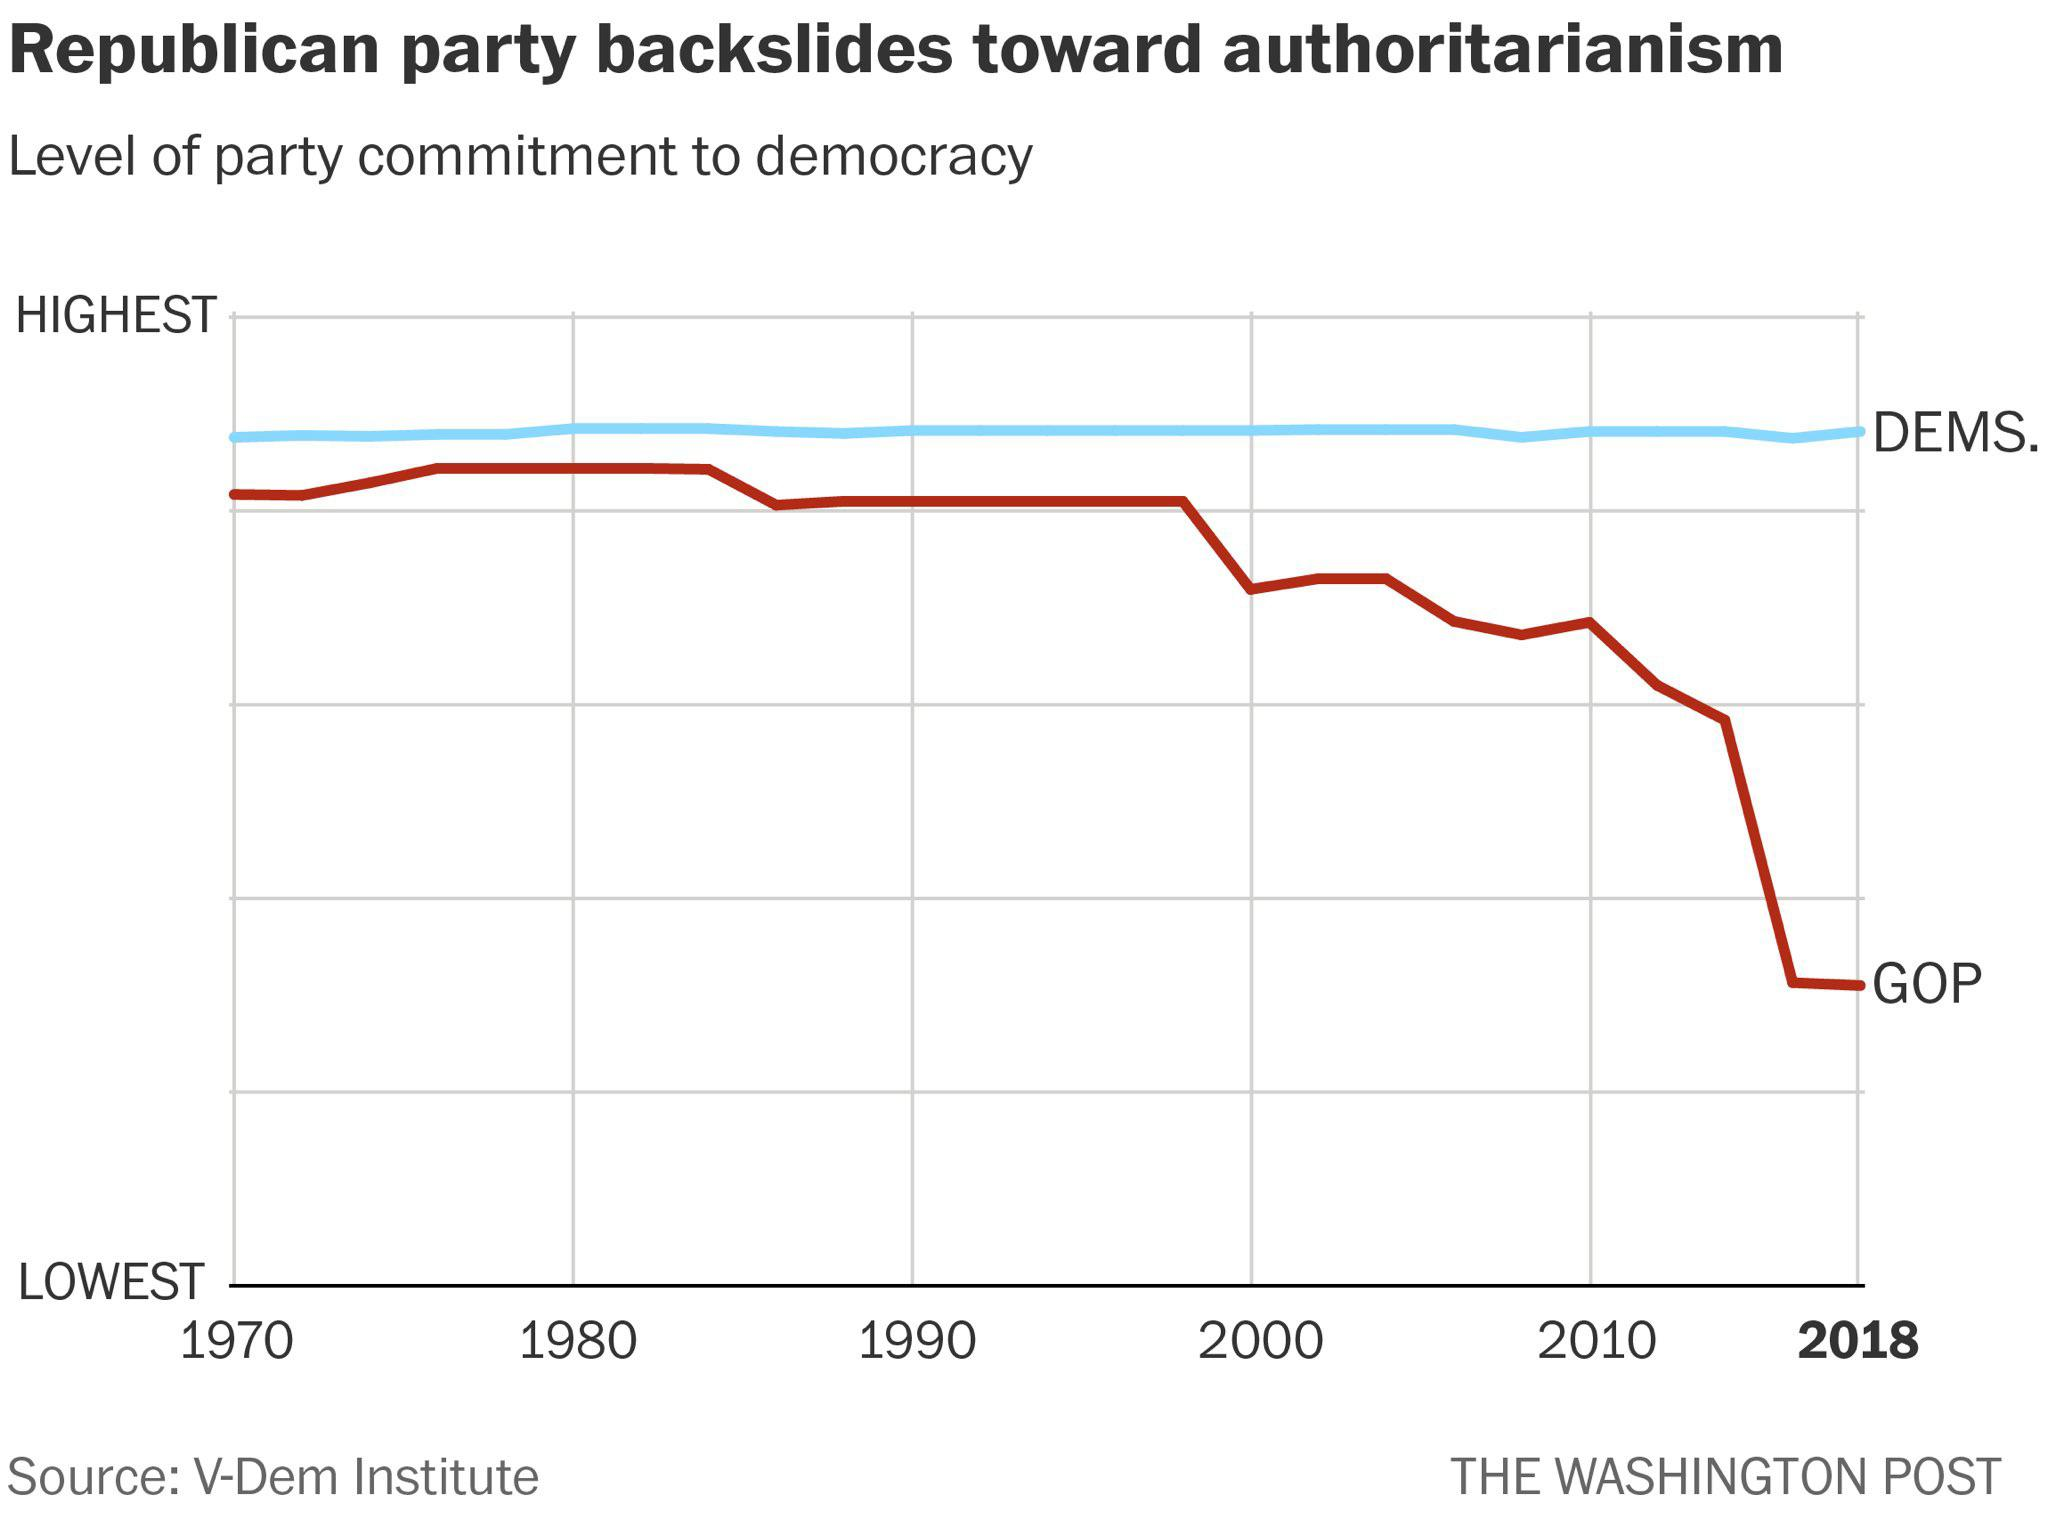
\includegraphics[height=60mm]{fig5/error-axis1.jpg} \\
	\scriptsize \ehref{https://www.reddit.com/r/dataisugly/comments/13hdd6j}{reddit.com/r/dataisugly/comments/13hdd6j}
\end{center}
\vfill
\end{frame}


\begin{frame}
\frametitle{Faxen mit Achsen}

\vfill
\begin{center}
	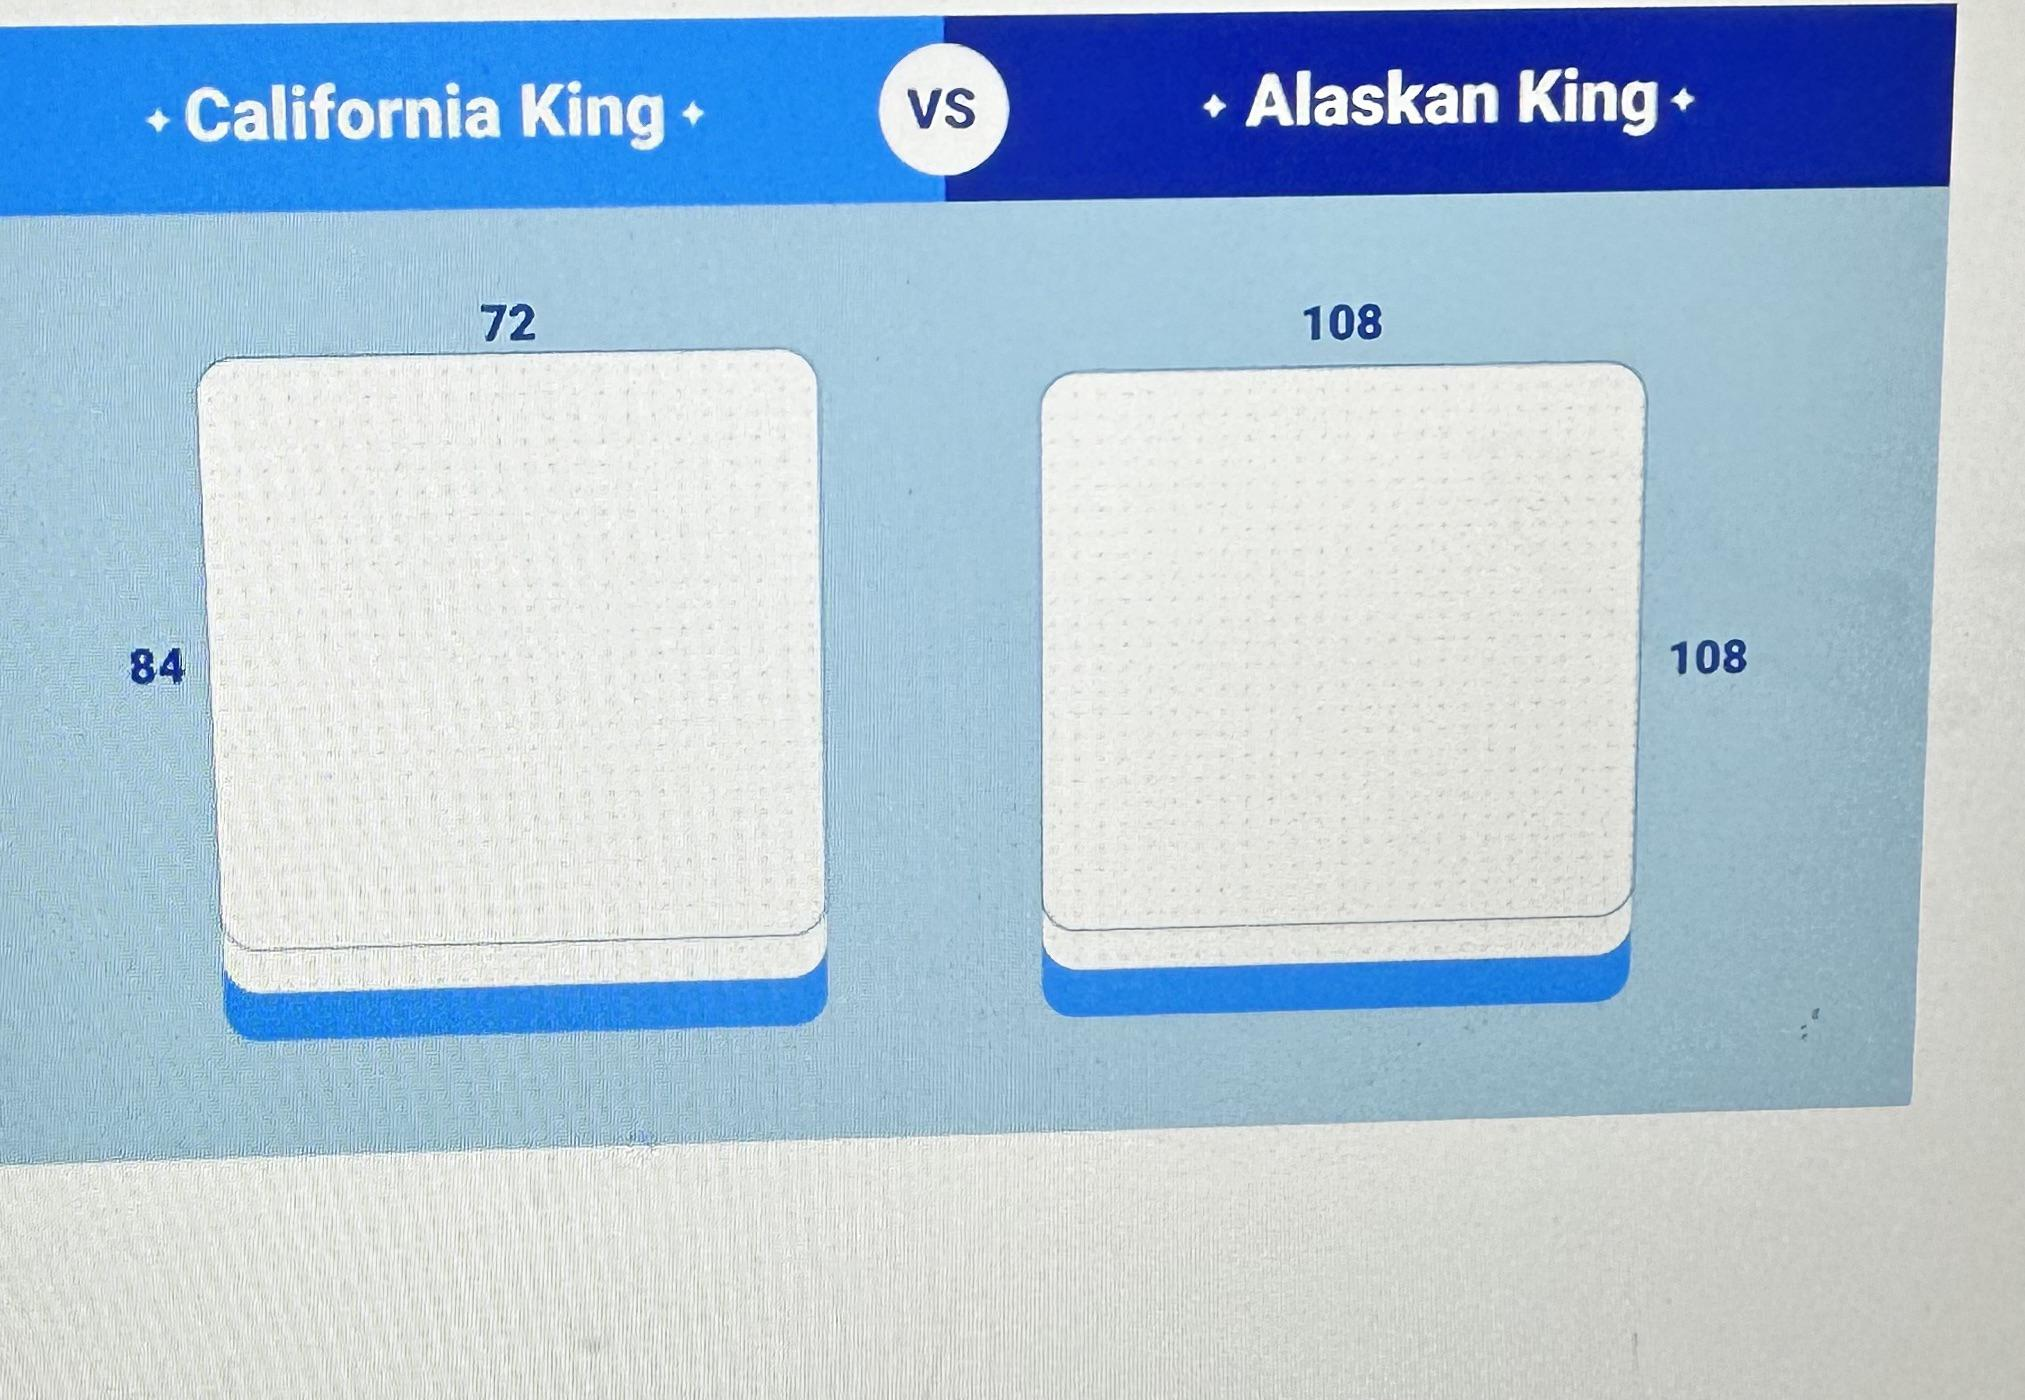
\includegraphics[height=60mm]{fig5/error-scale1.jpg} \\
	\scriptsize \ehref{https://www.reddit.com/r/dataisugly/comments/13mjvt3}{reddit.com/r/dataisugly/comments/13mjvt3}
\end{center}
\vfill
\end{frame}


\begin{frame}
\frametitle{Falscher Diagrammtyp}

\vfill
\begin{center}
	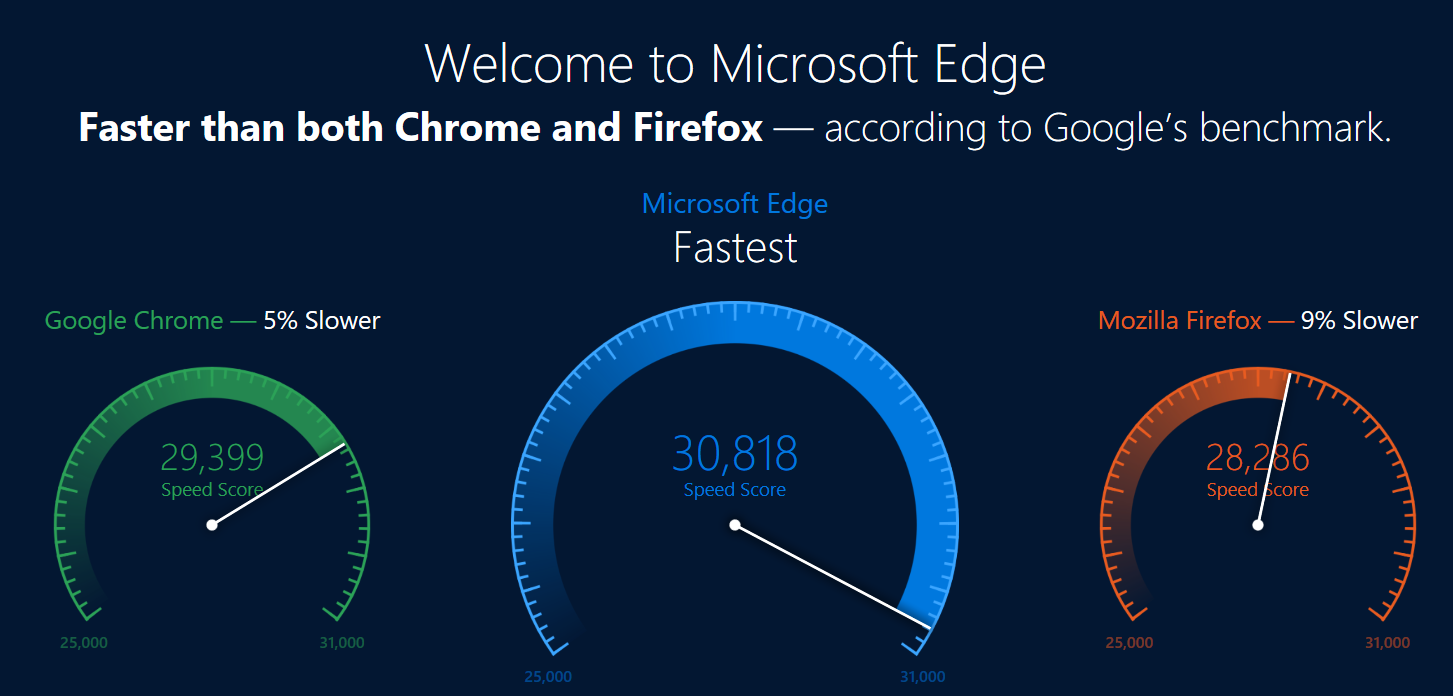
\includegraphics[height=50mm]{fig5/error-wrongtype.png} \\
	\scriptsize \ehref{https://www.reddit.com/r/dataisugly/comments/6sktdw}{reddit.com/r/dataisugly/comments/6sktdw}
\end{center}
\vfill
\end{frame}


\begin{frame}
\frametitle{Falscher Diagrammtyp}

\vfill
\begin{center}
	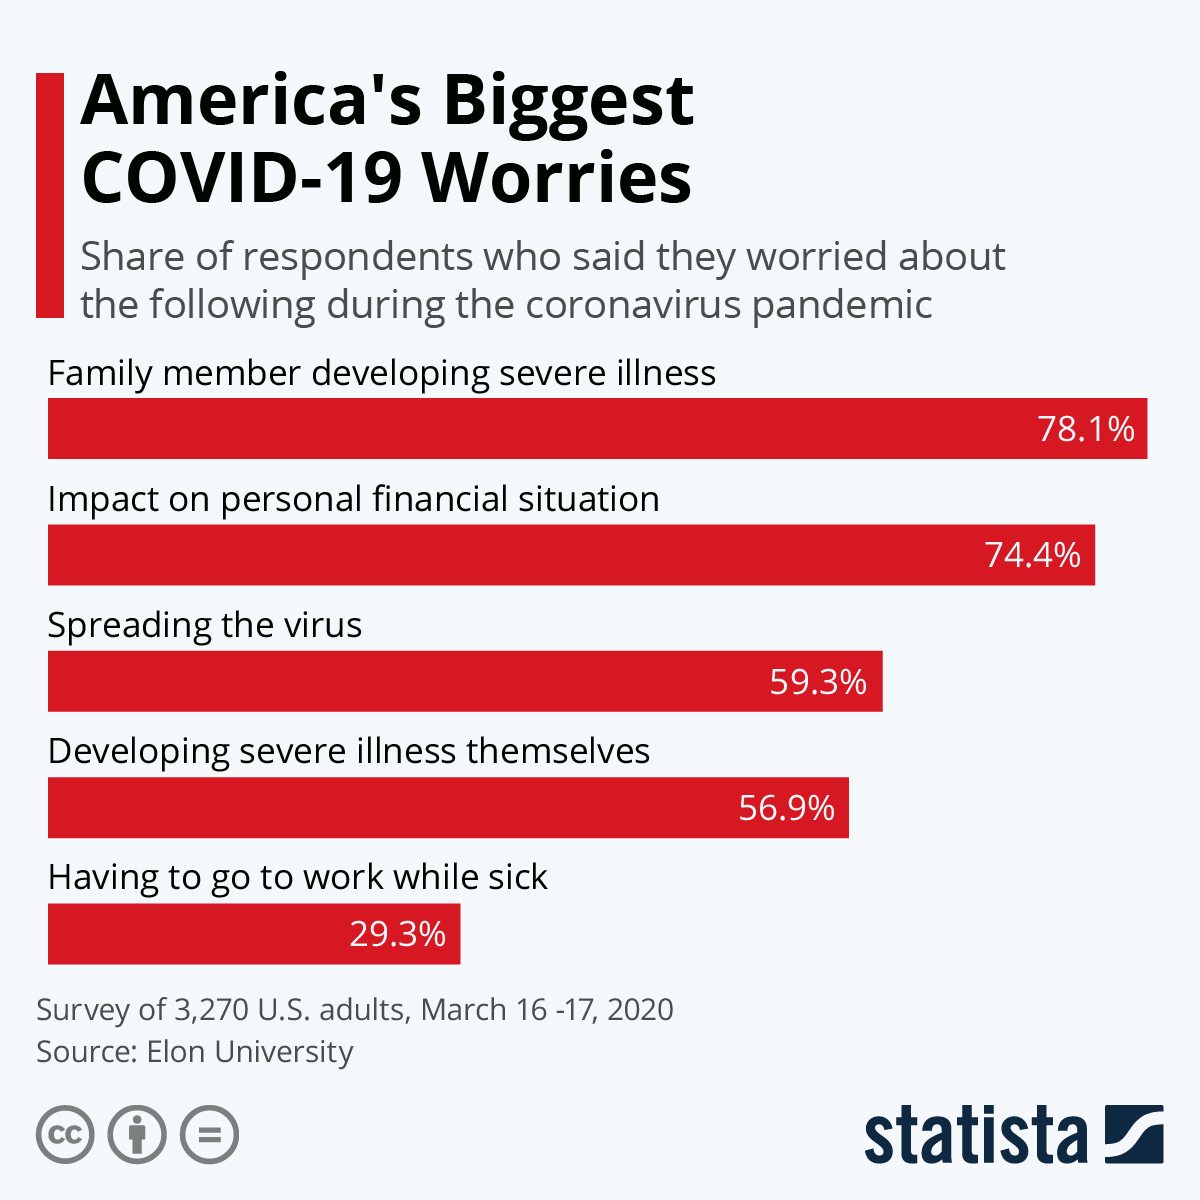
\includegraphics[height=60mm]{fig5/error-wrongtype2.jpg} \\
	\scriptsize \ehref{https://www.statista.com/chart/21193/worries-of-americans-covid-19/}{statista.com/chart/21193/worries-of-americans-covid-19}
\end{center}
\vfill
\end{frame}


\begin{frame}
\frametitle{Unterbrechung der Kontinuität}

\vfill
\begin{center}
	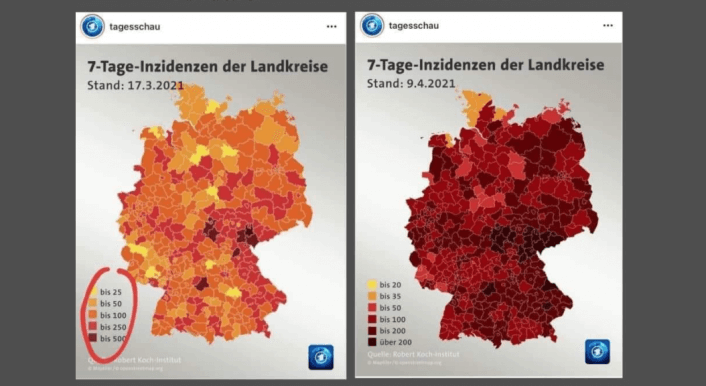
\includegraphics[height=60mm, clip, trim=22mm 0mm 22mm 2mm]{fig5/error-skalierung2.png}
	\scriptsize \ehref{https://correctiv.org/faktencheck/2021/04/14/diese-tagesschau-karten-zeigen-verschiedene-darstellungen-der-inzidenzwerte-fuer-tv-und-online/}{correctiv.org}
\end{center}
\vfill
\end{frame}


\begin{frame}
\frametitle{\dots{} und so weiter}

\begin{itemize}
	\item Überfrachten von Diagrammen
	\item Cherry-Picking
	\item \dots
\end{itemize}

\vspace{1cm}

Besuchen Sie doch mal
\begin{itemize}
	\item \ehref{https://www.reddit.com/r/dataisugly}{/r/dataisugly}
	\item \ehref{https://www.reddit.com/r/dataisbeautiful/}{/r/dataisbeautiful}
\end{itemize}
\end{frame}
